\chapter{Datos franceses}

Como adelantaba en la introducción, la tercera parte de este trabajo consiste concretamente en el modelado estadístico de los datos franceses que permitan la exploración de las configuraciones sociales que favorecieron o inhibieron el voto por el \textit{Front National} en las elecciones Presidenciales y Legislativas de 2007 y 2012. Por lo mismo, debo iniciar presentando dichos datos y realizando un análisis exploratorio; ese es el objetivo de este capítulo.\\

No obstante, antes de comenzar con el análisis exploratorio de datos, vale la pena decir que la unidad básica de estudio son las \textit{comunas} pues el objetivo del modelado es explorar \textit{configuraciones sociales}. Es decir, no estaré enfocándome en el nivel de individuo sino en los niveles de \textit{colectividades territoriales} de Francia. Como recordatorio de la {\color{Red} sección de división territorial francesa}, los 3 niveles administrativos de Francia son, en órden de jerarquía, las regiones, los departamentos y las comunas; es decir, una comuna pertenece a un departamento, que a su vez pertenece a una región.\\ 

\section{Datos electorales}

En las elecciones de 2007 la derecha fue la ganadora, como puede verse en los \textbf{Cuadros \ref{tbl:Resul_Oficiales_P07} y \ref{tbl:Resul_Oficiales_L07}}. En primer lugar, Nicolas Sarkozy obtuvo la presidencia con el 53.06\% de los votos en la segunda vuelta, frente a la candidata socialista Ségolène Royal. En las elecciones legislativas, ya con Sarkozy como presidente electo, su partido, el UMP, obtuvo 313 escaños en la Asamblea Nacional; además 22 diputados electos compitieron bajo la etiqueta de Mayoría Presidencial. Por su parte, Jean-Marie Le Pen como candidato presidencial frontista en 2007 obtuvo 10.44\% de la votación efectiva en la primera vuelta, quedando en cuarta posición y fuera de la segunda vuelta. Asimismo, el FN no logró conseguir ningún diputado a pesar de obtener más de 1 millón de votos en las primeras vueltas.\\ 

\begin{table}[h]
\centering
\resizebox{\linewidth}{!}{
\begin{tabular}{l c r r r r}
\multicolumn{6}{c}{\textbf{Elecciones Presidenciales 2007}} \\[5pt] 
\multirow{2}{*}{\textbf{Candidatura}} & 
\multirow{2}{*}{\textbf{Partido}} & 
\multicolumn{1}{c}{\textbf{Votos}} & \textbf{\% Ef.} & 
\multicolumn{1}{c}{\textbf{Votos}} & \textbf{\% Ef.}\\ 
& &  
\multicolumn{2}{c}{1ra vuelta} & 
\multicolumn{2}{c}{2da vuelta} \\[2pt] 
\hline
 & & & & & \\[\dimexpr-\normalbaselineskip+3pt]
Nicolas Sarkozy & UMP & 11,448,663 & 31.18 & 18,983,138 & 53.06 \\
Ségolène Royal & PS & 9,500,112 & 25.87 & 16,790,440 & 46.94\\
\hdashline
François Bayrou & UDF & 6,820,119 & 18.57 & & \\
Jean Marie Le Pen & FN & 3,834,530 & 10.44 & & \\
Olivier Besancenot & LRO & 1,498,581 & 4.08 & & \\
Philippe de Villiers & MPF & 818,407 & 2.23 & & \\
Marie-George Buffet & PC & 707,268 & 1.93 & & \\
Dominique Voynet & Verts & 576,666 & 1.57 & & \\
Arlette Laguiller & LO & 487,857 & 1.33 & & \\
José Bové & Indep. & 483,008 & 1.32 & & \\
Frédérick Nihous & CPNT & 420,645 & 1.15 & & \\
Gérard Schivardi & PT & 123,540 & 0.34 & & \\[3pt]
\hline
 & & & & & \\[\dimexpr-\normalbaselineskip+3pt]
\multicolumn{2}{l}{\textbf{Votación efectiva}} 
& 36,719,396 &
& 35,773,578 & \\
\multicolumn{2}{l}{Blancos o nulos} 
& 534,846 & 
& 1,568,426 & \\[3pt]
\hline
 & & & & & \\[\dimexpr-\normalbaselineskip+3pt]
\multicolumn{2}{l}{\textbf{Votación emitida}} 
& 37,254,242 & 
& 37,342,004 & \\
\multicolumn{2}{l}{Abstenciones} 
& 7,218,592 & 
& 7,130,729 & \\[3pt]
\hline
 & & & & & \\[\dimexpr-\normalbaselineskip+3pt]
\multicolumn{2}{l}{\textbf{Lista nominal}} 
& 44,472,834 & 
& 44,472,733 & \\
\end{tabular}
}
\caption{Resultados de las elecciones presidenciales francesas de 2007, resultando presidente electo Nicolas Sarkozy (UMP). Fuente: elaboración propia con los datos oficiales del Ministerio del Interior.}
\label{tbl:Resul_Oficiales_P07}
\end{table}

\begin{sidewaystable}[ph!]
\centering
\resizebox{\linewidth}{!}{
\begin{tabular}{l c r r c r r c c}
\multicolumn{9}{c}{\textbf{Elecciones Legislativas 2007}} \\[5pt] 
\multicolumn{2}{c}{\multirow{2}{*}{\textbf{Plataforma política}}} & 
\textbf{Votos} & 
\textbf{\% Ef.} & 
\textbf{Asientos} &
\textbf{Votos} & 
\textbf{\% Ef.} & 
\textbf{Asientos} &
\multirow{2}{*}{\textbf{Total de Asientos}}\\ 
\multicolumn{2}{c}{} 
& \multicolumn{3}{c}{1ra vuelta} 
& \multicolumn{3}{c}{2da vuelta} 
& \\[2pt] 
\hline
 & & & & & & & &\\[\dimexpr-\normalbaselineskip+3pt]
Union pour un Mouvement Populaire & UMP 
& 10,289,737 & 39.54 & 98 & 9,460,710 & 46.36 & 215 & 313 \\
Socialiste & SOC 
& 6,436,520 & 24.73 & 1 & 8,624,861 & 42.27 & 185 & 186 \\
Majorité Présidentielle & MAJ
& 616,440 & 2.37 & 8 & 433,057 & 2.12 & 14 & 22\\
Parti Communiste Français & COM 
& 1,115,663 & 4.29 & - & 464,739 & 2.28 & 15 & 15\\
Divers Gauche & DVG
& 513,407 & 1.97 & - & 503,556 & 2.47 & 15 & 15\\
Divers Droite & DVD 
& 641,842 & 2.47 & 2 & 238,588 & 1.17 & 7 & 9\\
Radicales de Gauche & RDG
& 343,565 & 1.32 & - & 333,194 & 1.63 & 7 & 7\\
Les Verts & VEC
& 845,977 & 3.25 & - & 90,975 & 0.45 & 4 & 4\\
Union pour la Démocratie Française & UDFD 
& 1,981,107 & 7.61 & - & 100,115 & 0.49 & 3 & 3\\
Mouvement pour la France & MPF
& 312,581 & 1.20 & 1 & - & - & - & 1\\
Divers & DIV 
& 267,760 & 1.03 & - & 33,068 & 0.16 & 1 & 1\\
Régionaliste & REG
& 133,473 & 0.51 & - & 106,484 & 0.52 & 1 & 1\\
Front National & FN 
& 1,116,136 & 4.29 & - & 17,107 & 0.08 & - & -\\
Extrême Gauche & EXG 
& 888,250 & 3.41 & - & -  & - & - & -\\
Chase Pêche Nature Traditions & CPNT 
& 213,427 & 0.82 & - & - & - & - & -\\
Ecologistes & ECO 
& 208,456 & 0.80 & - & - & - & - & -\\
Extrême Droite & EXD 
& 102,124 & 0.39 & - & - & - & - & -\\[3pt]
\hline
 & & & & & & & & \\[\dimexpr-\normalbaselineskip+3pt]
\multicolumn{2}{l}{\textbf{Votación efectiva}} 
& 26,026,465 & &
& 20,406,454 & & & \\
\multicolumn{2}{l}{Blancos o nulos} 
& 495,357 & &
& 722,585 & & & \\[3pt]
\hline
 & & & & & & & &\\[\dimexpr-\normalbaselineskip+3pt]
\multicolumn{2}{l}{\textbf{Votación emitida}} 
& 26,521,822 & &
& 21,129,039 & & & \\
\multicolumn{2}{l}{Abstenciones} 
& 17,374,011 & &
& 14,096,209 & & & \\[3pt]
\hline
 & & & & & & &\\[\dimexpr-\normalbaselineskip+3pt]
\multicolumn{2}{l}{\textbf{Lista nominal}} 
& 43,895,833 & &
& 35,225,248 & & & \\
\end{tabular}
}
\caption{Resultados de las elecciones legislativas de 2007 para el conjunto del territorio francés, incluyendo el ultramar. Fuente: elaboración propia con los datos oficiales del Ministerio del Interior.}
\label{tbl:Resul_Oficiales_L07}
\end{sidewaystable}

En 2012, sin embargo, Sarkozy perdió la reelección frente al socialista François Hollande, como puede verse en el \textbf{Cuadro \ref{tbl:Resul_Oficiales_P12}}. En el poder legislativo, la izquierda tomó el control del Hemiciclo gracias a los 280 diputados electos bajo las siglas del PS (\textbf{Cuadro \ref{tbl:Resul_Oficiales_L12}}). En lo que respecta al FN, este tuvo un crecimiento considerable. Con Marine Le Pen como lideresa y candidata, el partido obtuvo 17.90\% de la votación efectiva en la primera vuelta presidencial. Dicho porcentaje representó el 3er lugar en la elección, mejorando el 4to puesto de 2007. No obstante, de nueva cuenta fue insuficiente para disputar la segunda vuelta electoral. En las elecciones legislativas, sin embargo, el FN logró alrededor de 3 millones y medio de sufragios en la primera vuelta--- equivalentes al 13.60\%--- y consiguió 2 diputaciones.\\

\begin{table}[h]
\centering
\resizebox{\linewidth}{!}{
\begin{tabular}{l c r r r r}
\multicolumn{6}{c}{\textbf{Elecciones Presidenciales 2012}} \\[5pt] 
\multirow{2}{*}{\textbf{Candidato(a)}} & 
\multirow{2}{*}{\textbf{Partido}} & 
\multicolumn{1}{c}{\textbf{Votos}} & \textbf{\% Ef.} & 
\multicolumn{1}{c}{\textbf{Votos}} & \textbf{\% Ef.}\\ 
& &  
\multicolumn{2}{c}{1ra vuelta} & 
\multicolumn{2}{c}{2da vuelta} \\[2pt] 
\hline
 & & & & & \\[\dimexpr-\normalbaselineskip+3pt]
François Hollande & PS & 10,272,705 & 28.63 & 18,000,668 & 51.64\\
Nicolas Sarkozy & UMP & 9,753,629 & 27.18 & 16,860,685 & 48.36 \\
\hdashline
Marine Le Pen & FN & 6,421,426 & 17.90 & & \\
Jean-Luc Mélenchon & FG & 3,984,822 & 11.10 & & \\
François Bayrou & MoDem & 3,275,122 & 9.13 & & \\
Eva Joly & EELV & 828,345 & 2.31 & & \\
Nicolas Dupont-Aignan & DLR & 643,907 & 1.79 & & \\
Philippe Poutou & NPA & 411,160 & 1.15 & & \\
Nathalie Arthaud & LO & 202,548 & 0.56 & & \\
Jacques Cheminade & SP & 89,545 & 0.25 & & \\[3pt]
\hline
 & & & & & \\[\dimexpr-\normalbaselineskip+3pt]
\multicolumn{2}{l}{\textbf{Votación efectiva}} 
& 35,883,209 &
& 34,861,353 & \\
\multicolumn{2}{l}{Blancos o nulos} 
& 701,190 & 
& 2,154,956 & \\[3pt]
\hline
 & & & & & \\[\dimexpr-\normalbaselineskip+3pt]
\multicolumn{2}{l}{\textbf{Votación emitida}} 
& 36,584,399 & 
& 37,016,309 & \\
\multicolumn{2}{l}{Abstenciones} 
& 9,444,143 & 
& 9,049,998 & \\[3pt]
\hline
 & & & & & \\[\dimexpr-\normalbaselineskip+3pt]
\multicolumn{2}{l}{\textbf{Lista nominal}} 
& 46,028,542 & 
& 46,066,307 & \\
\end{tabular}
}
\caption{Resultados de las elecciones presidenciales francesas de 2012, resultando presidente electo François Hollande (PS). Fuente: elaboración propia con los datos oficiales del Ministerio del Interior.}
\label{tbl:Resul_Oficiales_P12}
\end{table}

\begin{sidewaystable}[ph!]
\centering
\resizebox{\linewidth}{!}{
\begin{tabular}{l c r r c r r c c}
\multicolumn{9}{c}{\textbf{Elecciones Legislativas 2012}} \\[5pt] 
\multicolumn{2}{c}{\multirow{2}{*}{\textbf{Plataforma política}}} & 
\textbf{Votos} & 
\textbf{\% Ef.} & 
\textbf{Asientos} &
\textbf{Votos} & 
\textbf{\% Ef.} & 
\textbf{Asientos} &
\multirow{2}{*}{\textbf{Total de Asientos}}\\ 
\multicolumn{2}{c}{} 
& \multicolumn{3}{c}{1ra vuelta} 
& \multicolumn{3}{c}{2da vuelta} 
& \\[2pt] 
\hline
 & & & & & & & &\\[\dimexpr-\normalbaselineskip+3pt]
Socialiste & SOC 
& 7,618,326 & 29.35 & 22 & 9,420,889 & 40.91 & 258 & 280 \\
Union pour un Mouvement Populaire & UMP 
& 7,037,268 & 27.12 & 9 & 8,740,628 & 37.95 & 185 & 194 \\
Divers Gauche & DVG
& 881,555 & 3.40 & 1 & 709,395 & 3.08 & 21 & 22\\
Europe-Écologie-Les Verts & VEC
& 1,418,264 & 5.46 & 1 & 829,036 & 3.60 & 16 & 17\\
Divers Droite & DVD 
& 910,034 & 3.51 & 1 & 417,940 & 1.81 & 14 & 15\\
Nouveau Centre & NCE
& 569,897 & 2.20 & 1 & 568,319 & 2.47 & 11 & 12\\
Radicales de Gauche & RDG
& 428,898 & 1.65 & 1 & 538,331 & 2.34 & 11 & 12\\
Front de Gauche & FG 
& 1,793,192 & 6.91 & - & 249,498 & 1.08 & 10 & 10\\
Parti Radical & PRV
& 321,124 & 1.24 & - & 311,199 & 1.35 & 6 & 6\\
Front National & FN 
& 3,528,663 & 13.60 & - & 842,695 & 3.66 & 2 & 2\\
Le Centre pour la France & CEN
& 458,098 & 1.77 & 1 & 113,196 & 0.49 & 2 & 2\\
Alliance Centriste & ALLI 
& 156,026 & 0.60 & - & 123,132 & 0.53 & 2 & 2\\
Régionaliste & REG
& 145,809 & 0.56 & - & 135,312 & 0.59 & 2 & 2\\
Extrême Droite & EXD 
& 49,499 & 0.19 & - & 29,738 & 0.13 & 1 & 1\\
Extrême Gauche & EXG 
& 253,386 & 0.98 & - & - & - & - & -\\
Ecologistes & ECO 
& 249,068 & 0.96 & - & - & - & - & -\\
Autres & AUT 
& 133,752 & 0.52 & - & - & - & - & -\\[3pt]
\hline
 & & & & & & & & \\[\dimexpr-\normalbaselineskip+3pt]
\multicolumn{2}{l}{\textbf{Votación efectiva}} 
& 25,952,859 & &
& 23,029,308 & & & \\
\multicolumn{2}{l}{Blancos o nulos} 
& 416,267 & &
& 923,178 & & & \\[3pt]
\hline
 & & & & & & & &\\[\dimexpr-\normalbaselineskip+3pt]
\multicolumn{2}{l}{\textbf{Votación emitida}} 
& 26,369,126 & &
& 23,952,486 & & & \\
\multicolumn{2}{l}{Abstenciones} 
& 19,712,978 & &
& 19,281,162 & & & \\[3pt]
\hline
 & & & & & & &\\[\dimexpr-\normalbaselineskip+3pt]
\multicolumn{2}{l}{\textbf{Lista nominal}} 
& 46,082,104 & &
& 43,233,648 & & & \\
\end{tabular}
}
\caption{Resultados de las elecciones legislativas de 2012 para el conjunto del territorio francés, incluyendo el ultramar. Fuente: elaboración propia con los datos oficiales del Ministerio del Interior.}
\label{tbl:Resul_Oficiales_L12}
\end{sidewaystable}

Ahora bien, como puede verificarse con las cuatro elecciones, en Francia existe una gran variedad de partidos políticos repartidos a lo largo del espectro político, tradicionalmente asociado con las nociones de izquierda y derecha. Adicionalmente, no es raro que los partidos cambien de nombres o formen coaliciones. Por ejemplo, en 2007 hubo 12 candidaturas presidenciales y para  2012 fueron 10. En las elecciones legislativas se presentaron 17 etiquetas políticas diferentes ambas ocasiones. Por ello, y para simplificar el análisis, conviene agrupar las diferentes opciones políticas bajo algunas etiquetas cualitativas generales.\\ 

Dependiendo de la posición--- aproximada--- de la plataforma política en el eje ideológico izquierda-derecha propondría los siguientes grupos. En primer lugar, debido al interés específico en el Front National, este es clasificado individualmente. Posteriormente, tenemos a los partidos tradicionales de derecha e izquierda--- el UMP\footnote{Este partido ya cambió de nombre y ahora se conoce como \textit{Les Republicains}. En 2007, después de que Nicolas Sarkozy ganara las elecciones, además de los candidatos del UMP hubo candidaturas bajo la etiqueta de la \textit{Mayoría presidencial} por lo que también las agrupo junto con el UMP.} y los socialistas del PS, respectivamente---. Además, existen plataformas de centro, así como otras izquierdas y derechas. Finalmente, encontramos opciones con un fuerte componente temático--- como los verdes o los regionalistas--- o con una plataforma política especial de forma tal que resulta más conveniente separarlos del eje y clasificarlos en una categoría residual. Así pues, en total existen 7 grupos generales: 

\begin{itemize}
\item FN
\item Derecha
\item Izquierda
\item Centro
\item Otras derechas
\item Otras izquierdas
\item Otros
\end{itemize}

En las \textbf{Figuras \ref{fig:Partidos_07} y \ref{fig:Partidos_12}} pueden observarse representaciones esquemáticas de esta simplificación del espectro político francés para 2007 y 2012, respectivamente.\\

\begin{figure}[h]
	\centering
	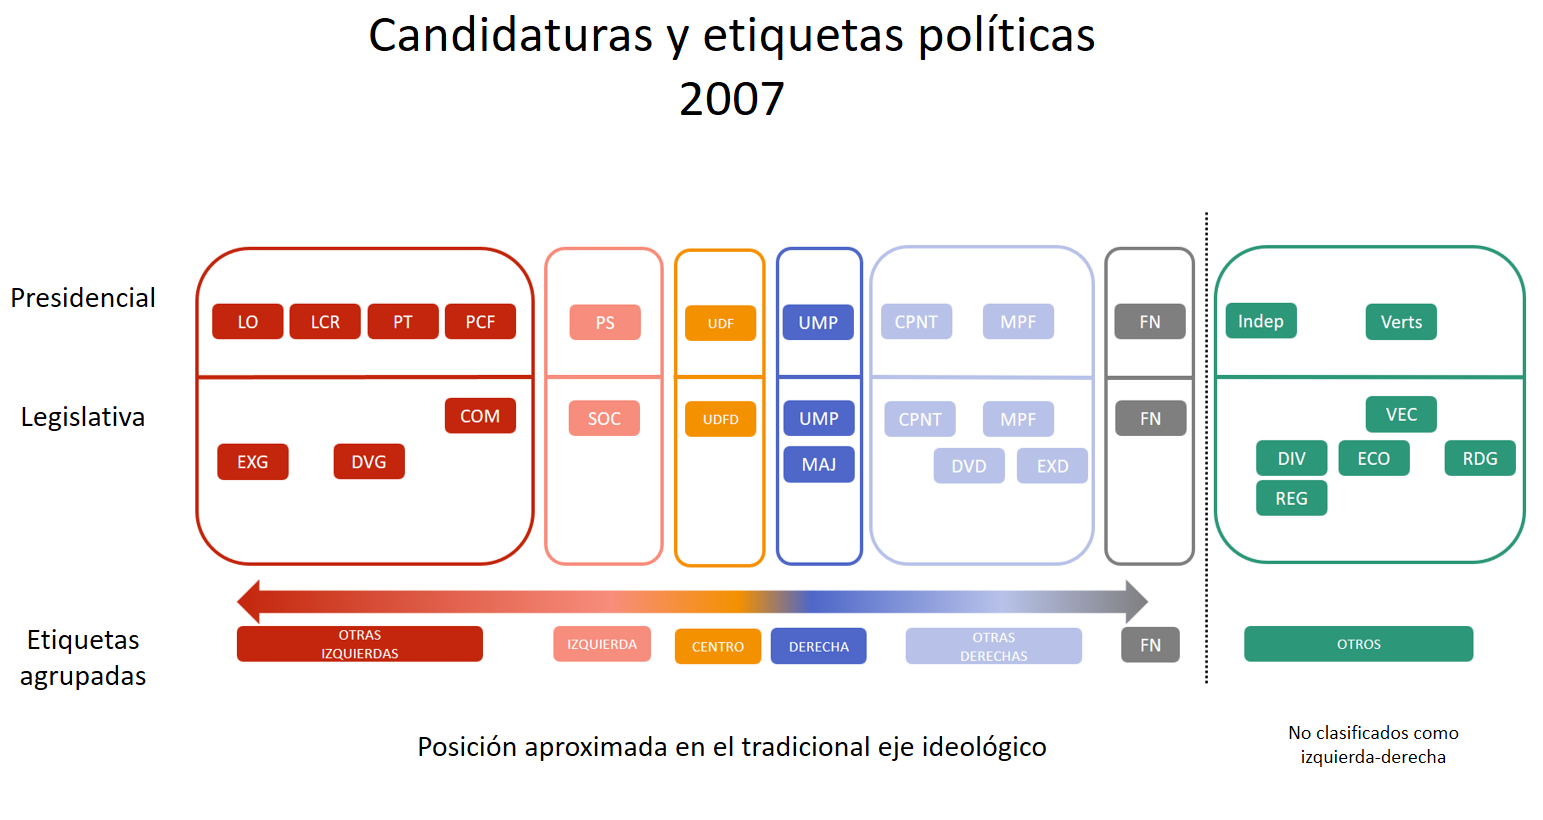
\includegraphics[width = 0.9\textwidth]{Figs/FN_Francia/Partidos_07}
	\caption{Representación esquemática de los partidos, candidaturas y etiquetas políticas en las elecciones francesas de 2007. Fuente: elaboración propia.}
	\label{fig:Partidos_07}	
\end{figure}

\begin{figure}[h]
	\centering
	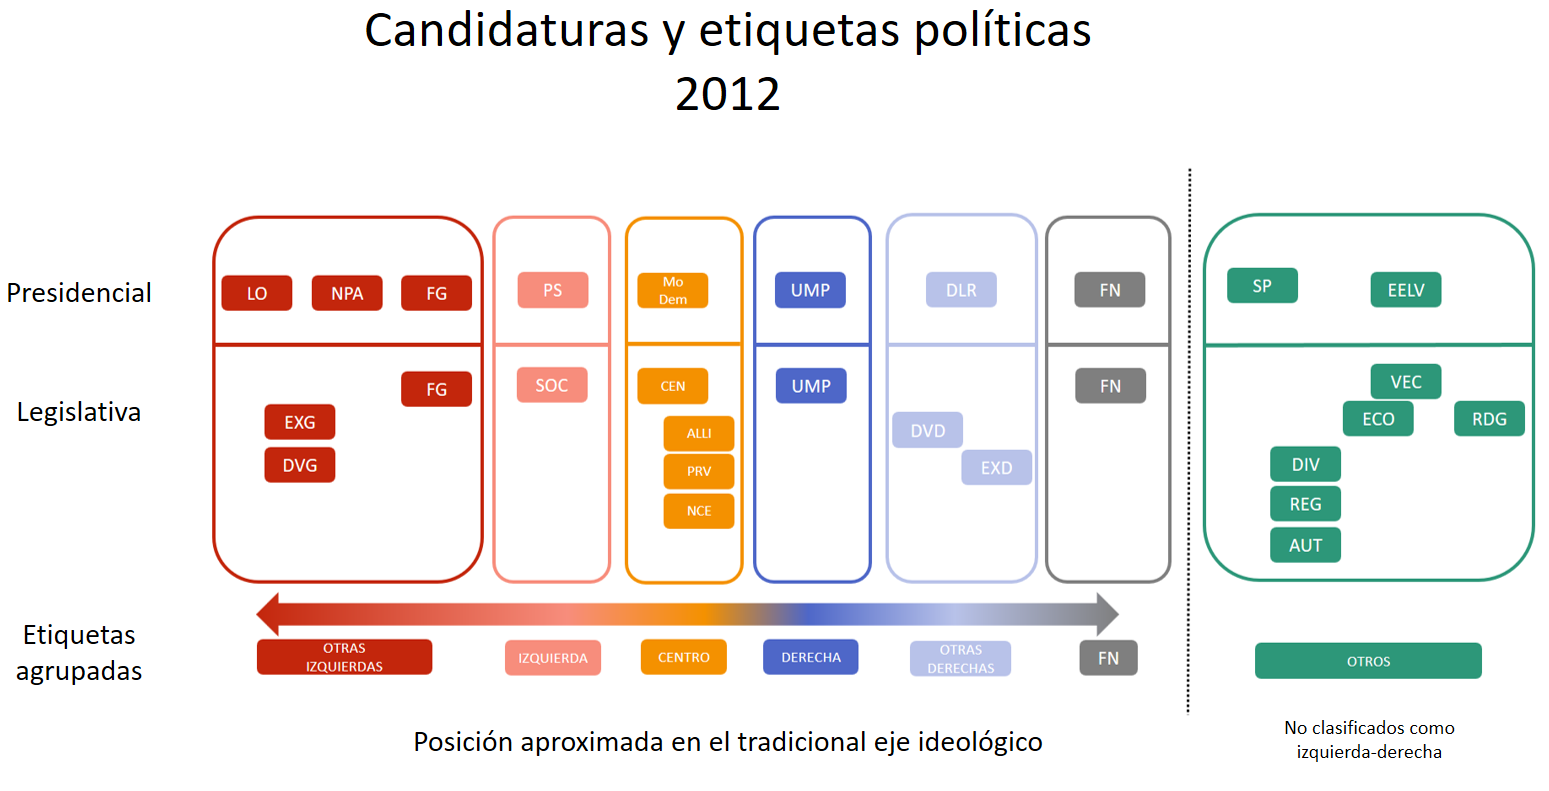
\includegraphics[width = 0.9\textwidth]{Figs/FN_Francia/Partidos_12}
	\caption{Representación esquemática de los partidos, candidaturas y etiquetas políticas en las elecciones francesas de 2007. Fuente: elaboración propia.}
	\label{fig:Partidos_12}	
\end{figure}

Debido a que el FN compitió primordialmente en las primeras vueltas en las 4 elecciones, solo me enfocaré en ellas y no en las segundas vueltas. Asimismo, el fenómeno electoral es marcadamente distinto en la metrópoli francesa que en los territorios de ultramar donde, naturalmente, el FN es prácticamente inexistente. Por tanto, el análisis también se circunscribe a los resultados dentro de la metrópoli francesa. En consecuencia, a partir de este momento, todos los resultados electorales se refieren a las primeras vueltas de las 4 elecciones sin considerar los territorios de ultramar.\\

Una vez mencionados los resultados generales de las 4 elecciones, hay que notar que la distribución geográfica de los votos no es uniforme. Existen zonas de fortaleza para los diferentes partidos. Una forma de observar esto es agrupar las comunas de cada región francesa y comparar la distribución del voto para cada etiqueta política en cada región frente a la distribución agregada de toda la metrópoli. Como ejemplo, podemos ver este ejercicio para la elección presidencial de 2012 mediante los \textit{geofacets} de la \textbf{Figura \ref{fig:Geofacet_Distr_Reg_P12}}. Cada \textit{geofacet} representa las distribuciones de voto de cada etiqueta política. Dentro de ellos comparo los histogramas de los porcentajes de votos que recibió la etiqueta política en las comunas de cada región con la distribución de los porcentajes para todas las comunas de la metrópoli. La intensidad del color de los histogramas depende del cociente del porcentaje mediano de votos en la región entre el porcentaje mediano de votos en toda la metrópoli, por lo que representa la fuerza relativa de cada etiqueta en la región.\\

\begin{figure}[h]
	\centering
	\begin{subfigure}{0.3\textwidth}
	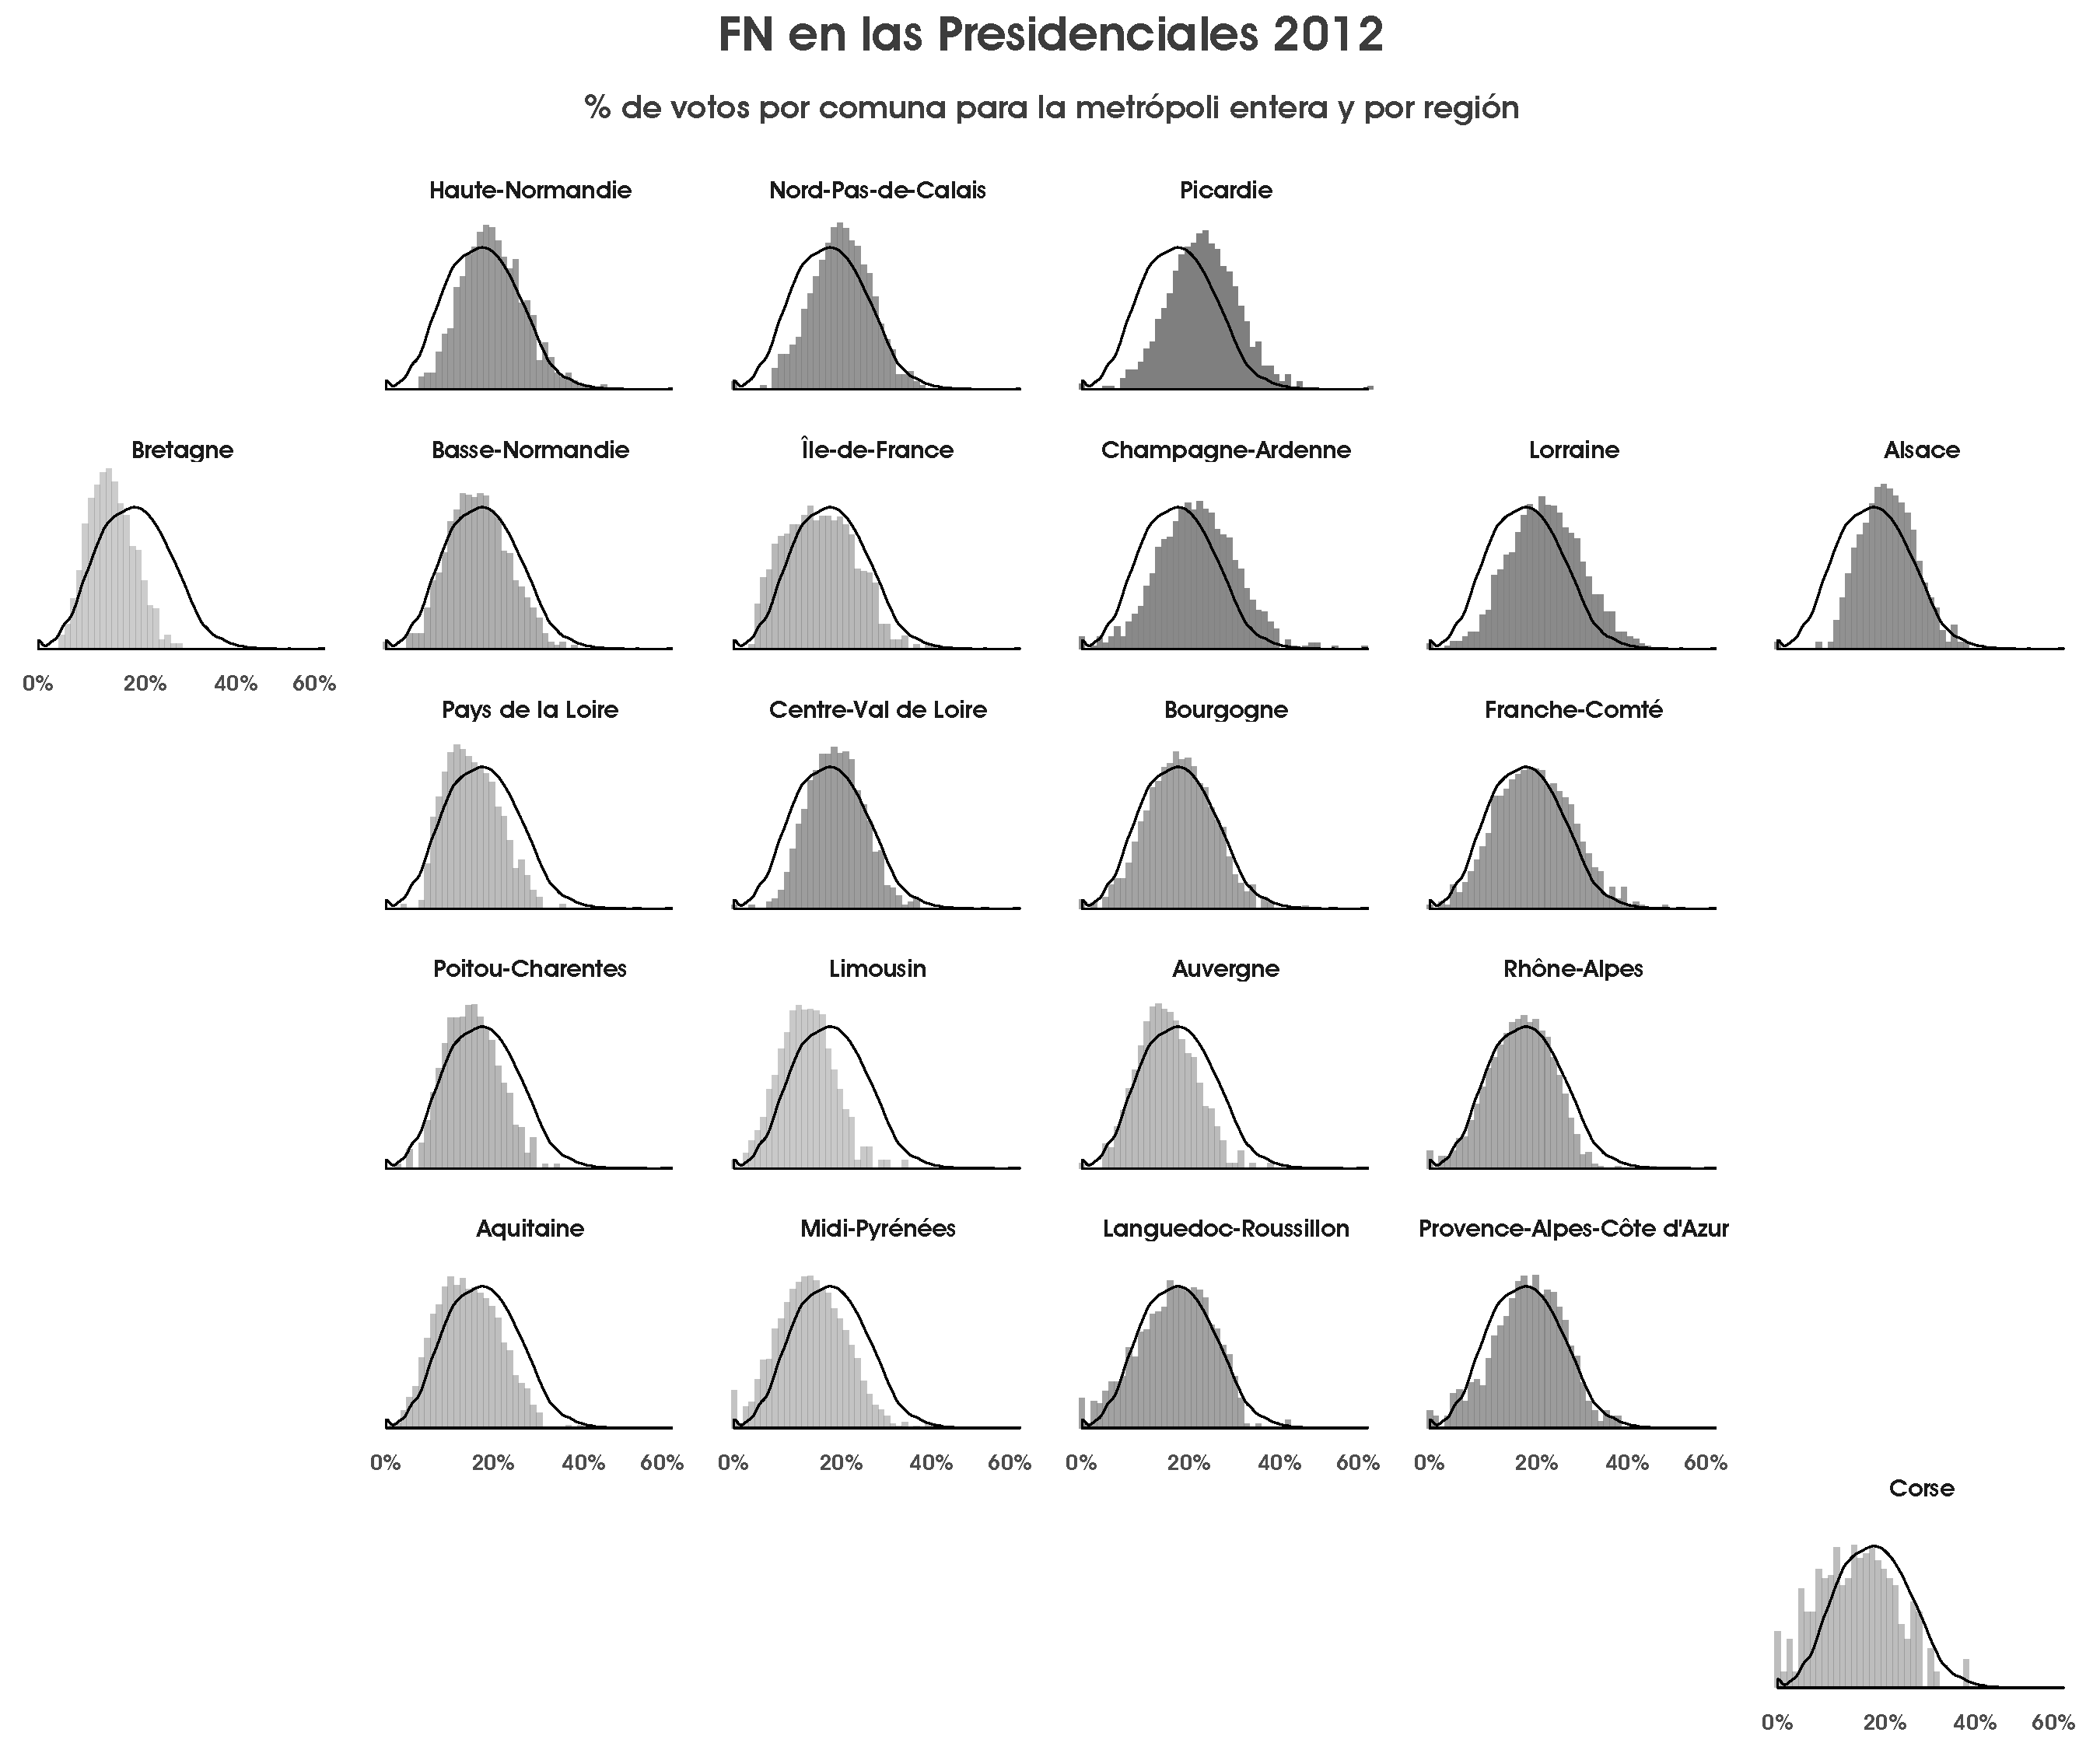
\includegraphics[width = \textwidth]{Figs/AED/Geofacet_Distr_por_Reg_P12_FN}
	\end{subfigure}\\	
	~
	\begin{subfigure}{0.3\textwidth}
	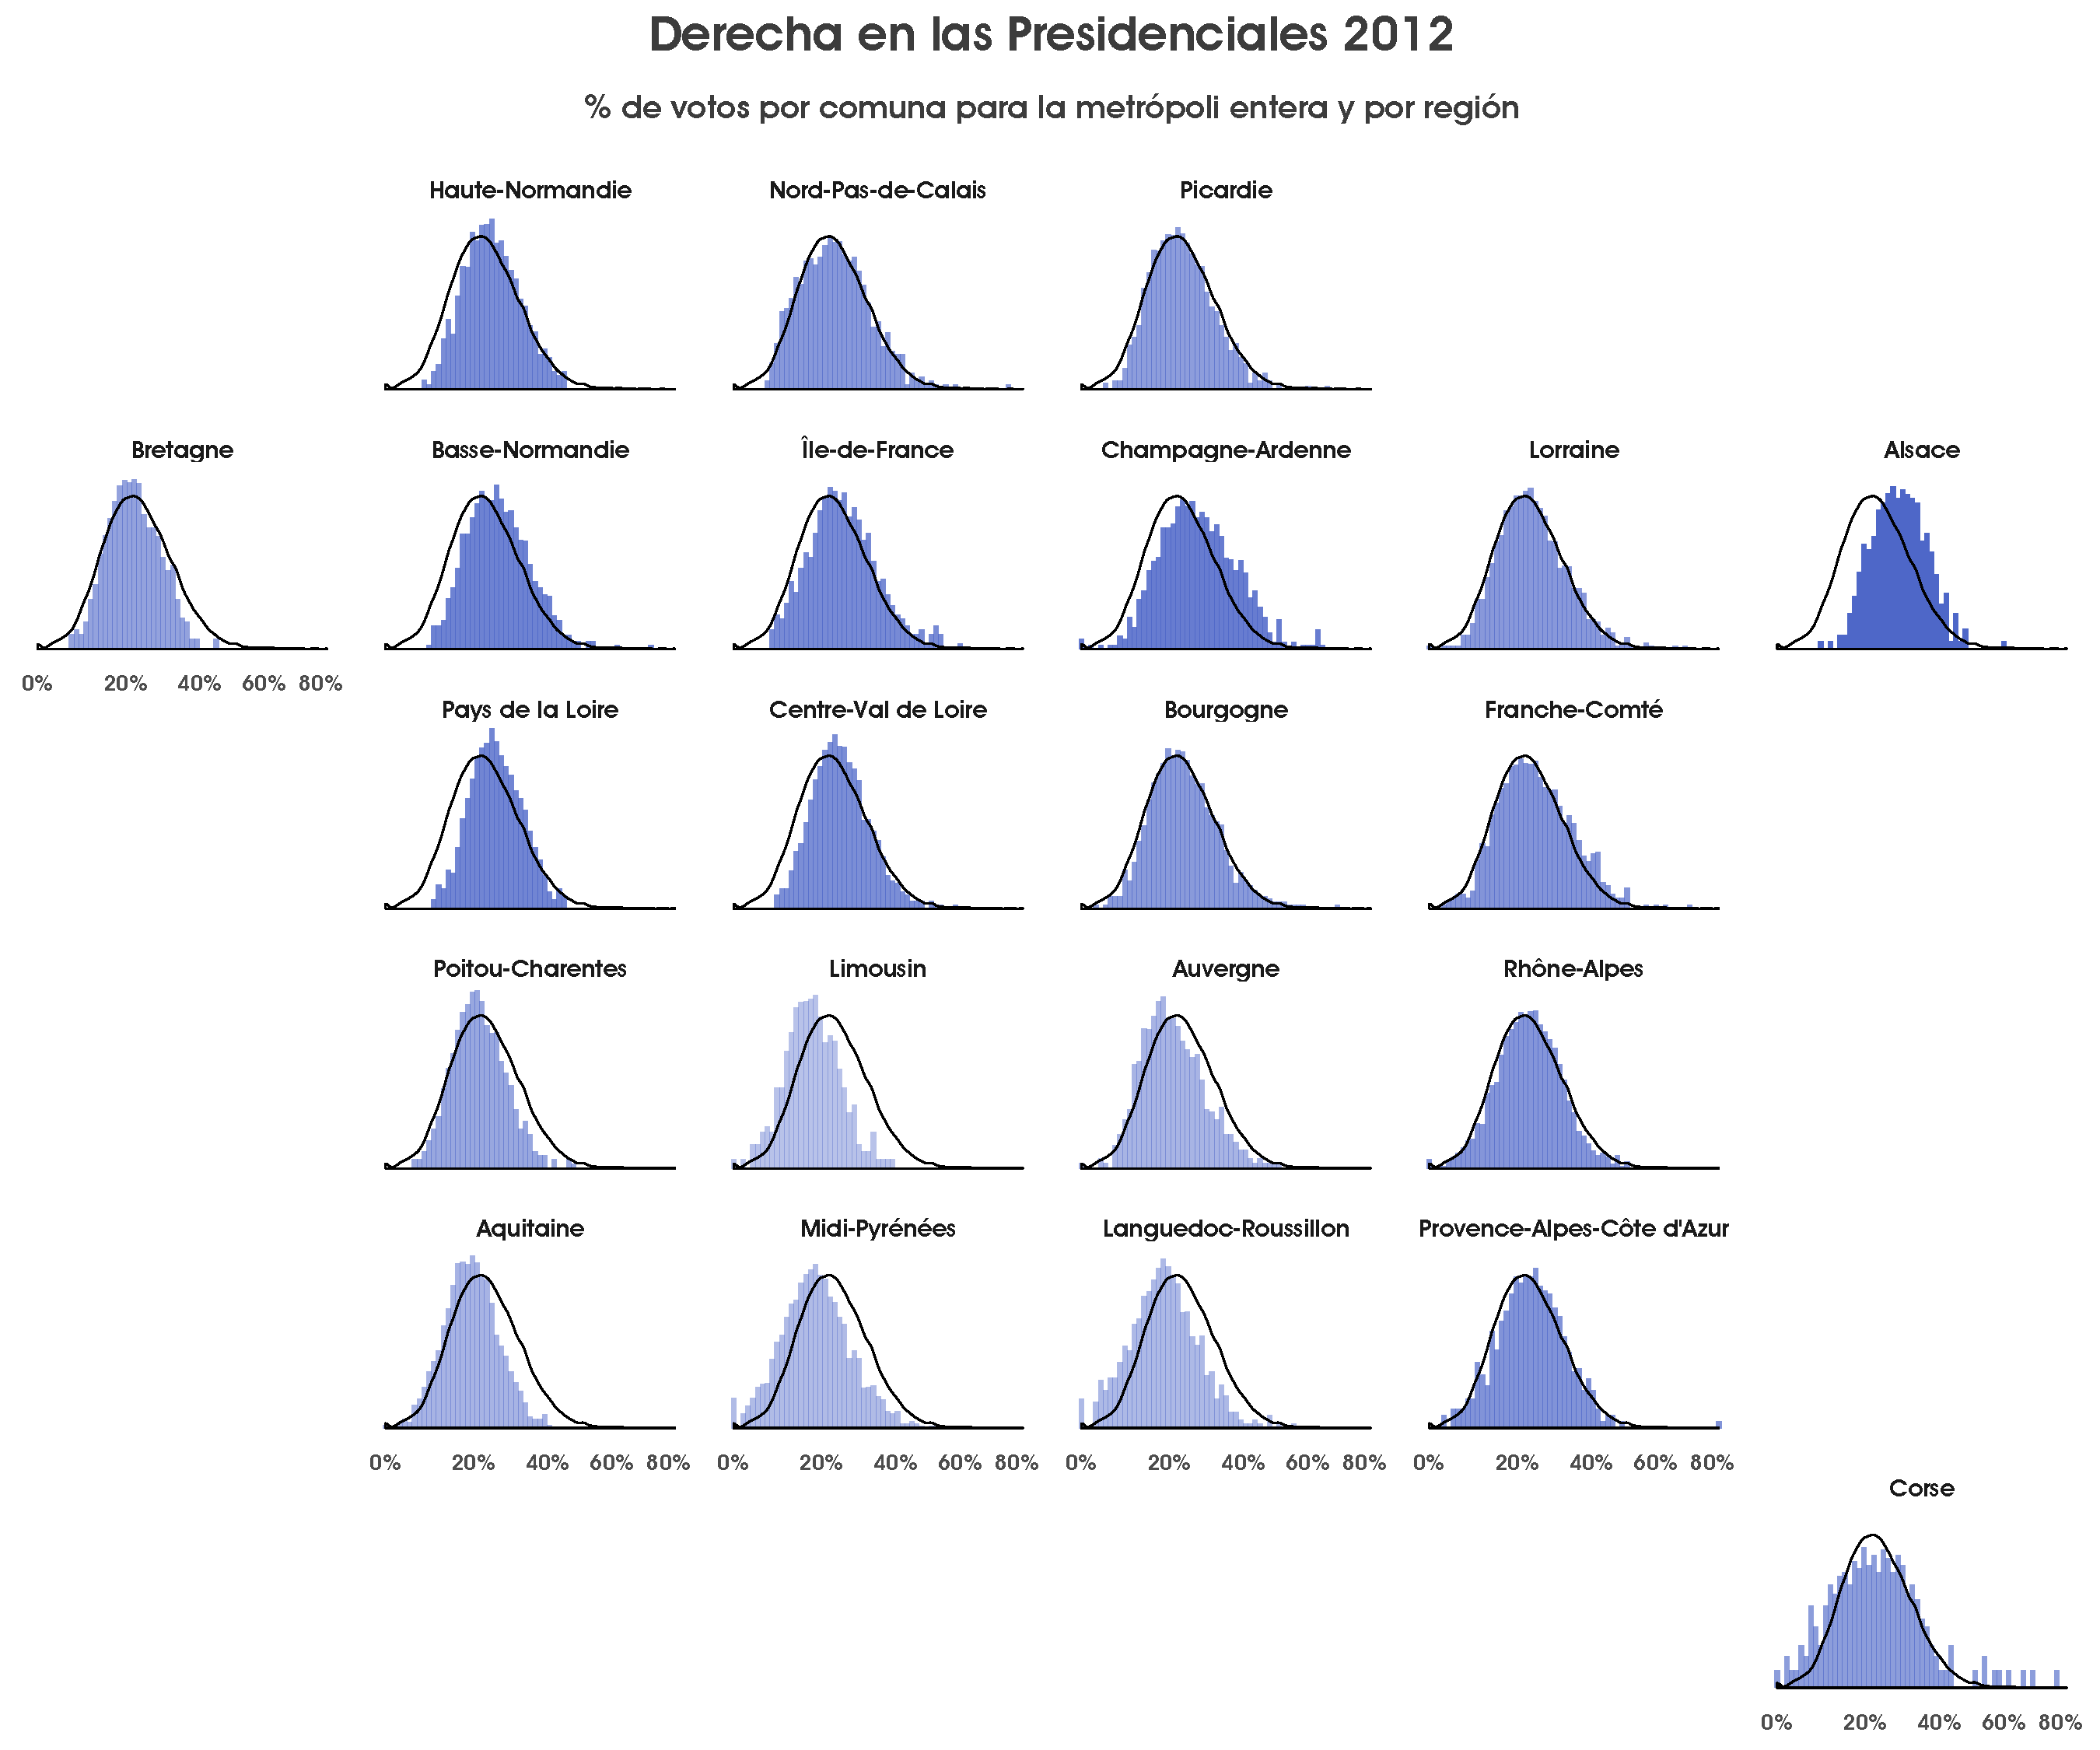
\includegraphics[width = \textwidth]{Figs/AED/Geofacet_Distr_por_Reg_P12_Derecha}
	\end{subfigure}
	~
	\begin{subfigure}{0.3\textwidth}
	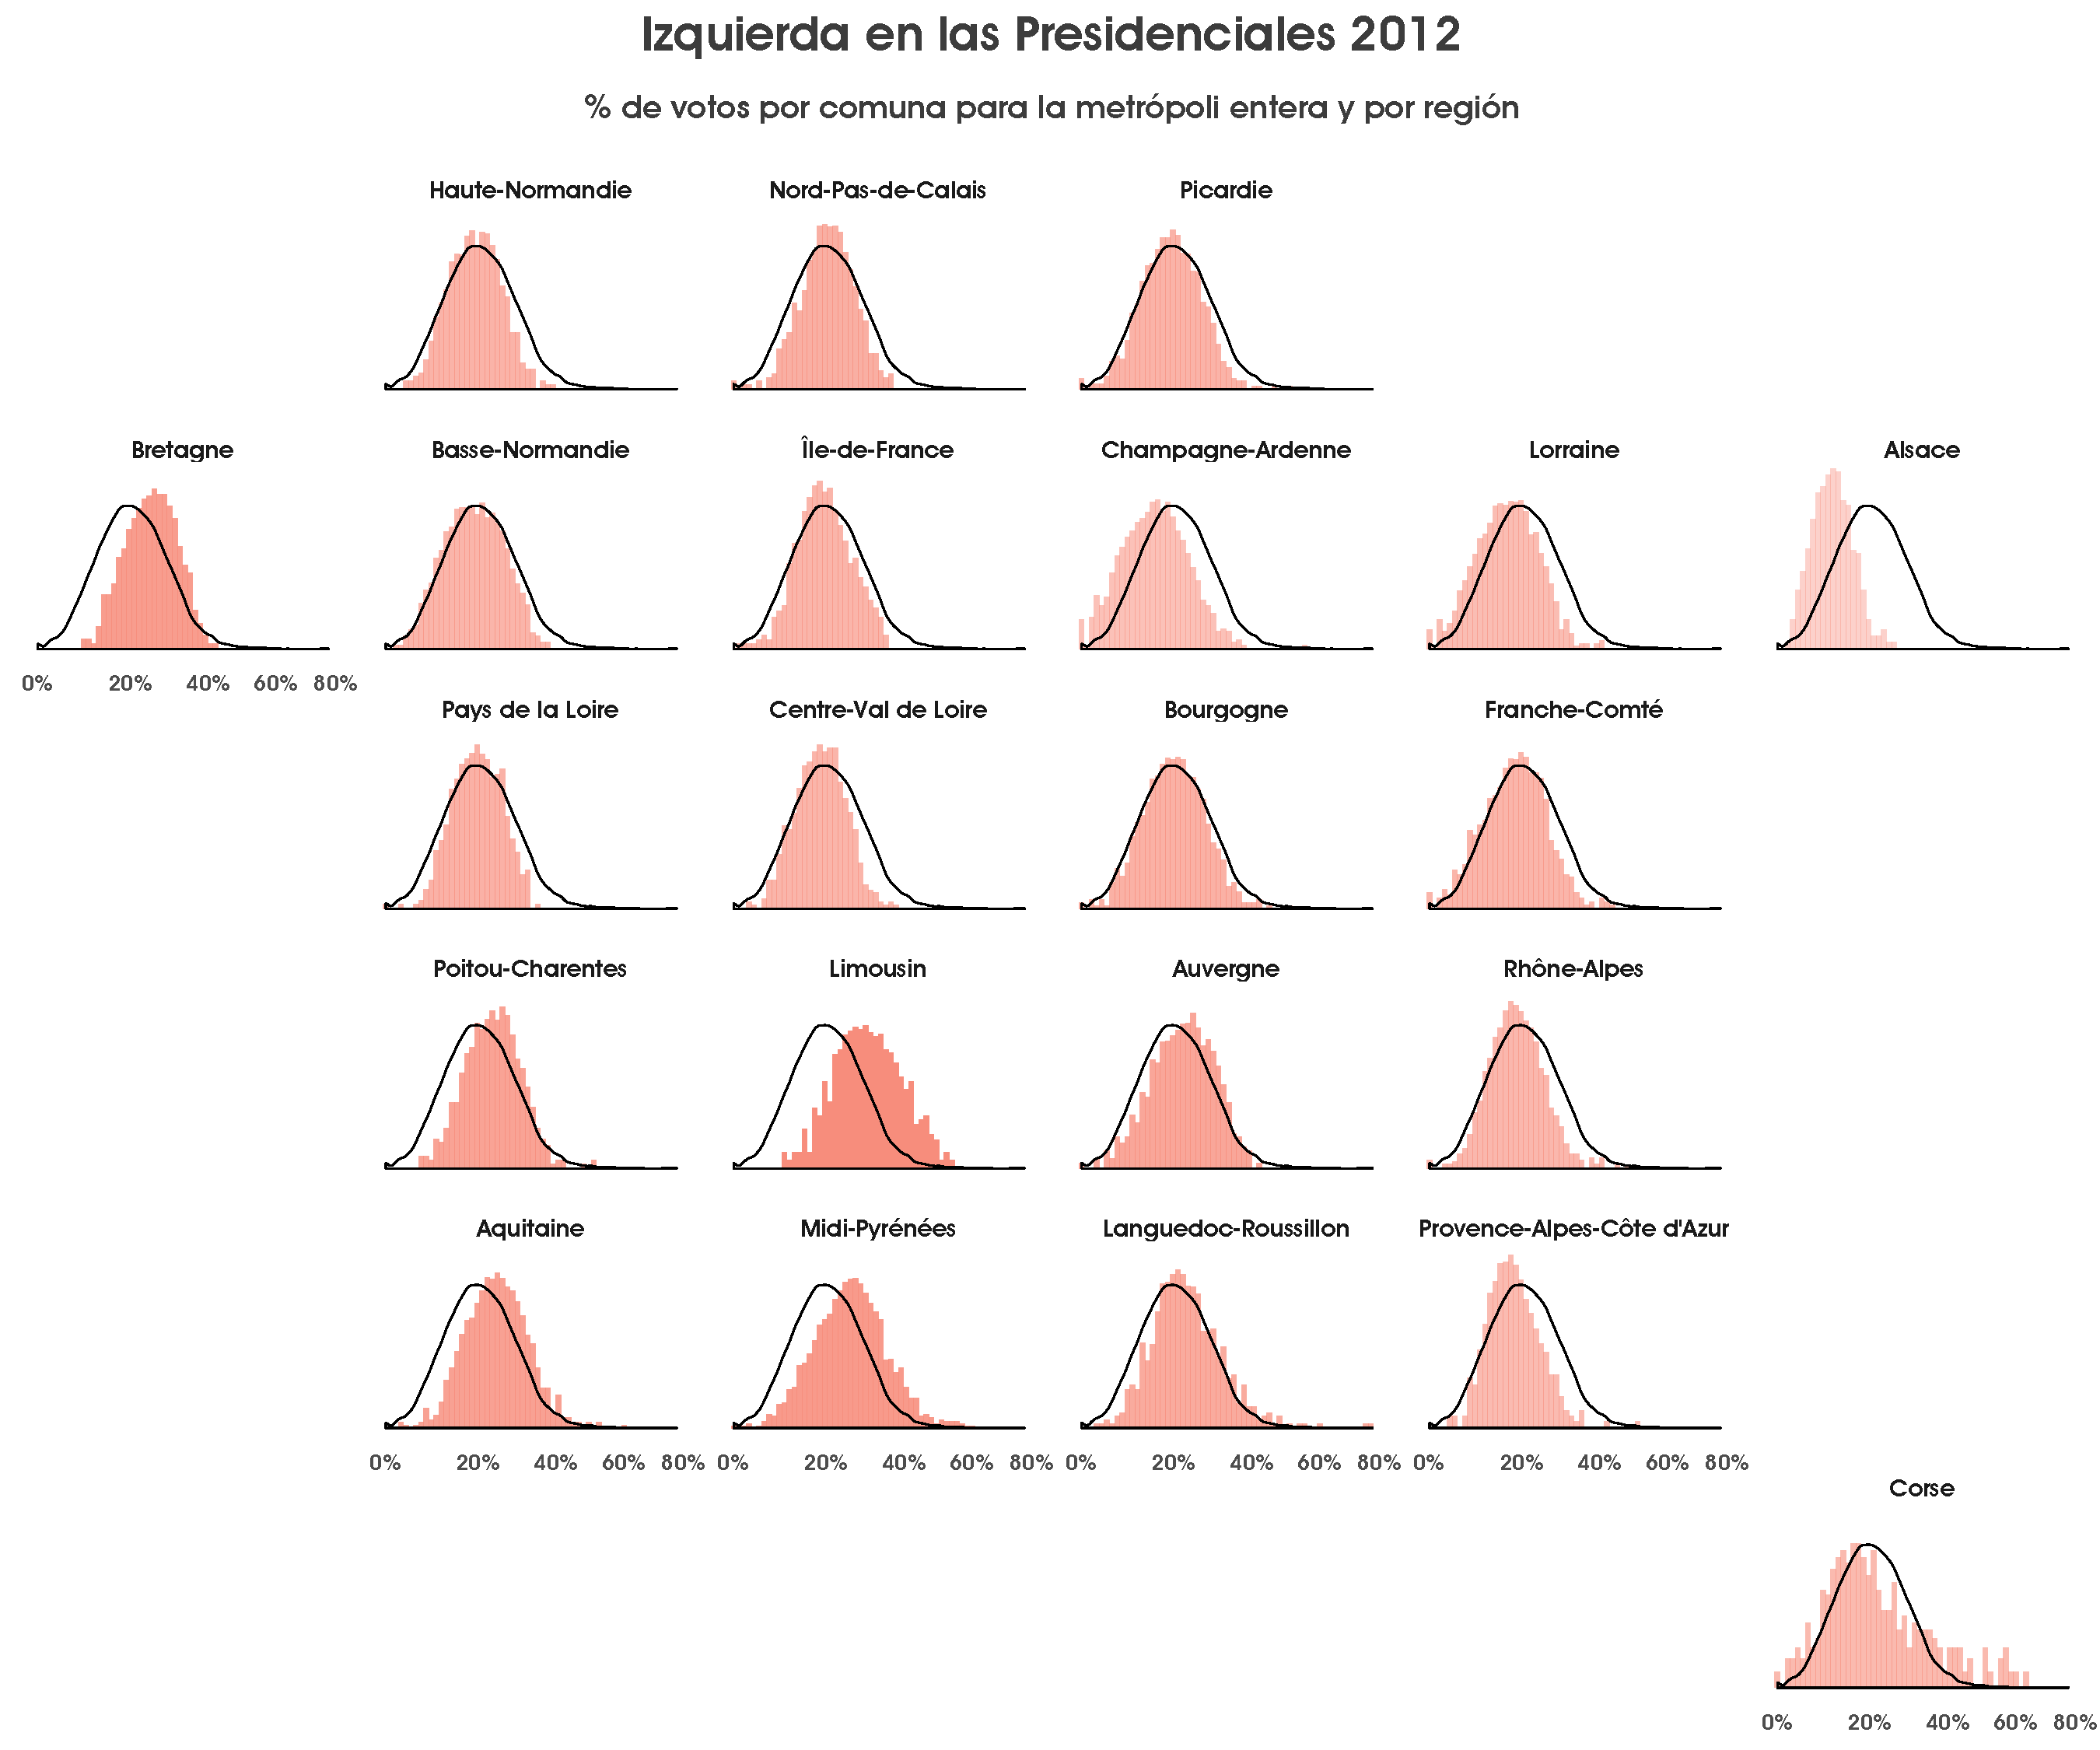
\includegraphics[width = \textwidth]{Figs/AED/Geofacet_Distr_por_Reg_P12_Izquierda}
	\end{subfigure}
	~
	\begin{subfigure}{0.3\textwidth}
	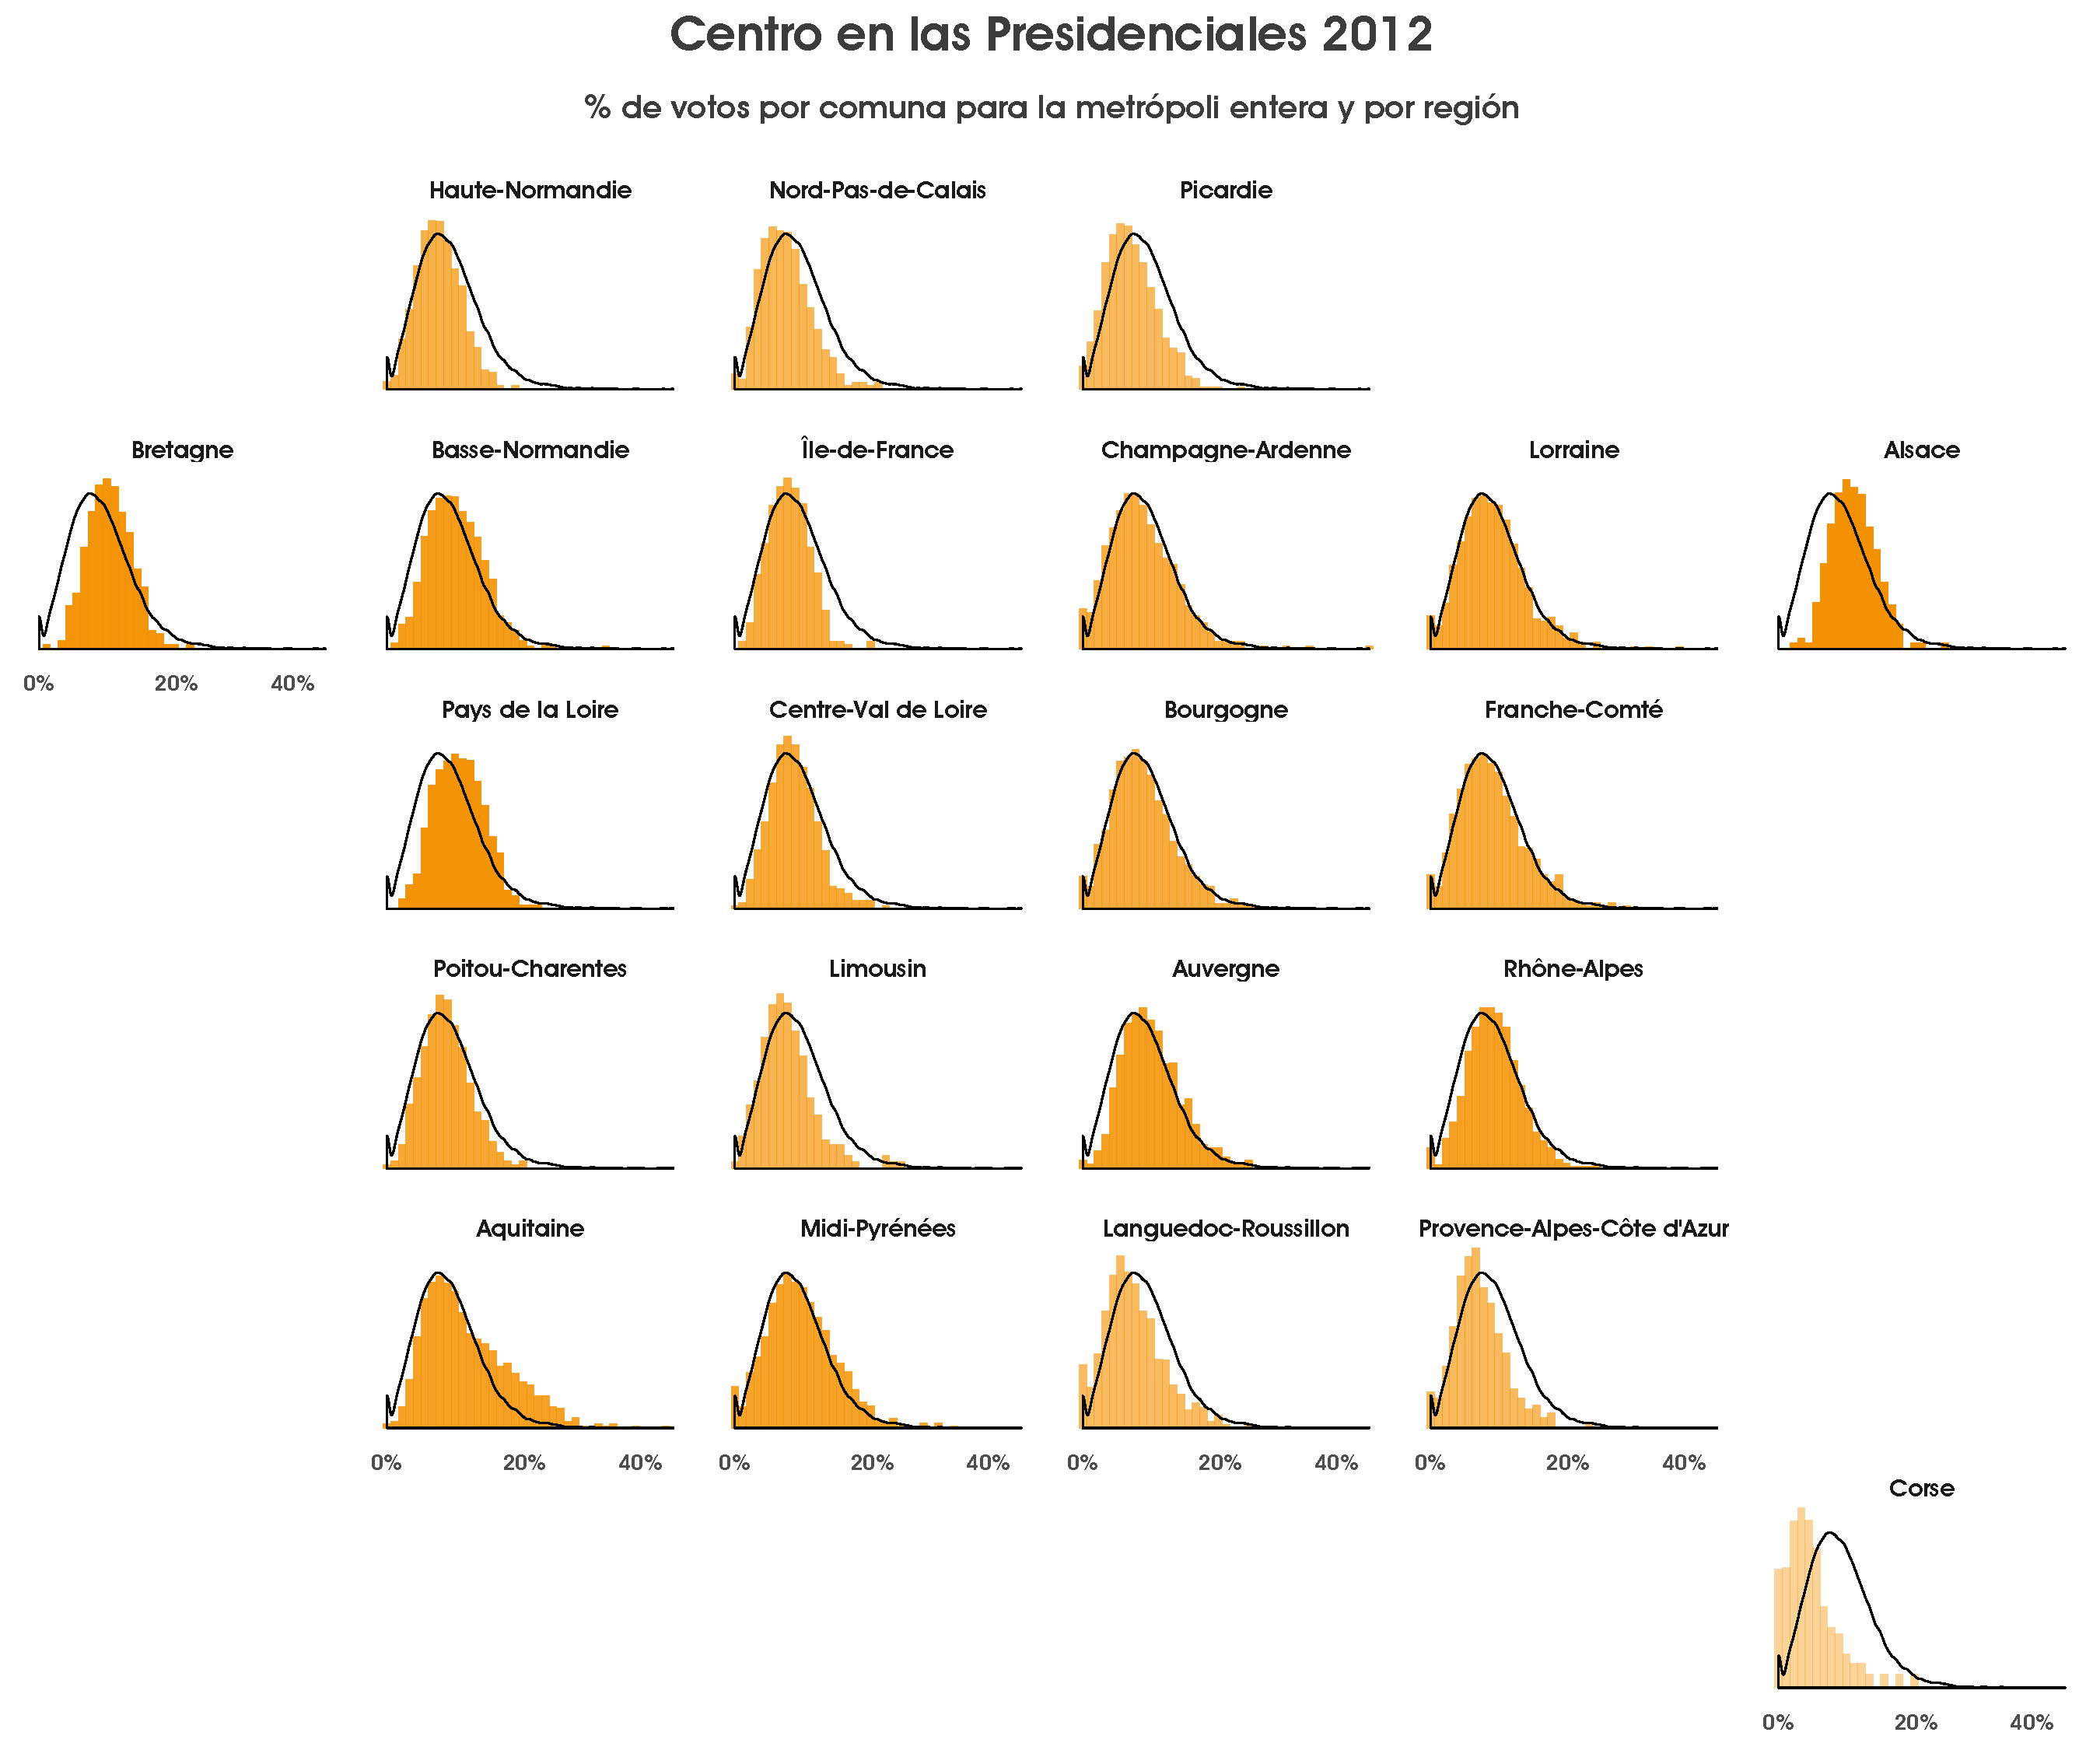
\includegraphics[width = \textwidth]{Figs/AED/Geofacet_Distr_por_Reg_P12_Centro}
	\end{subfigure}
	~
	\begin{subfigure}{0.3\textwidth}
	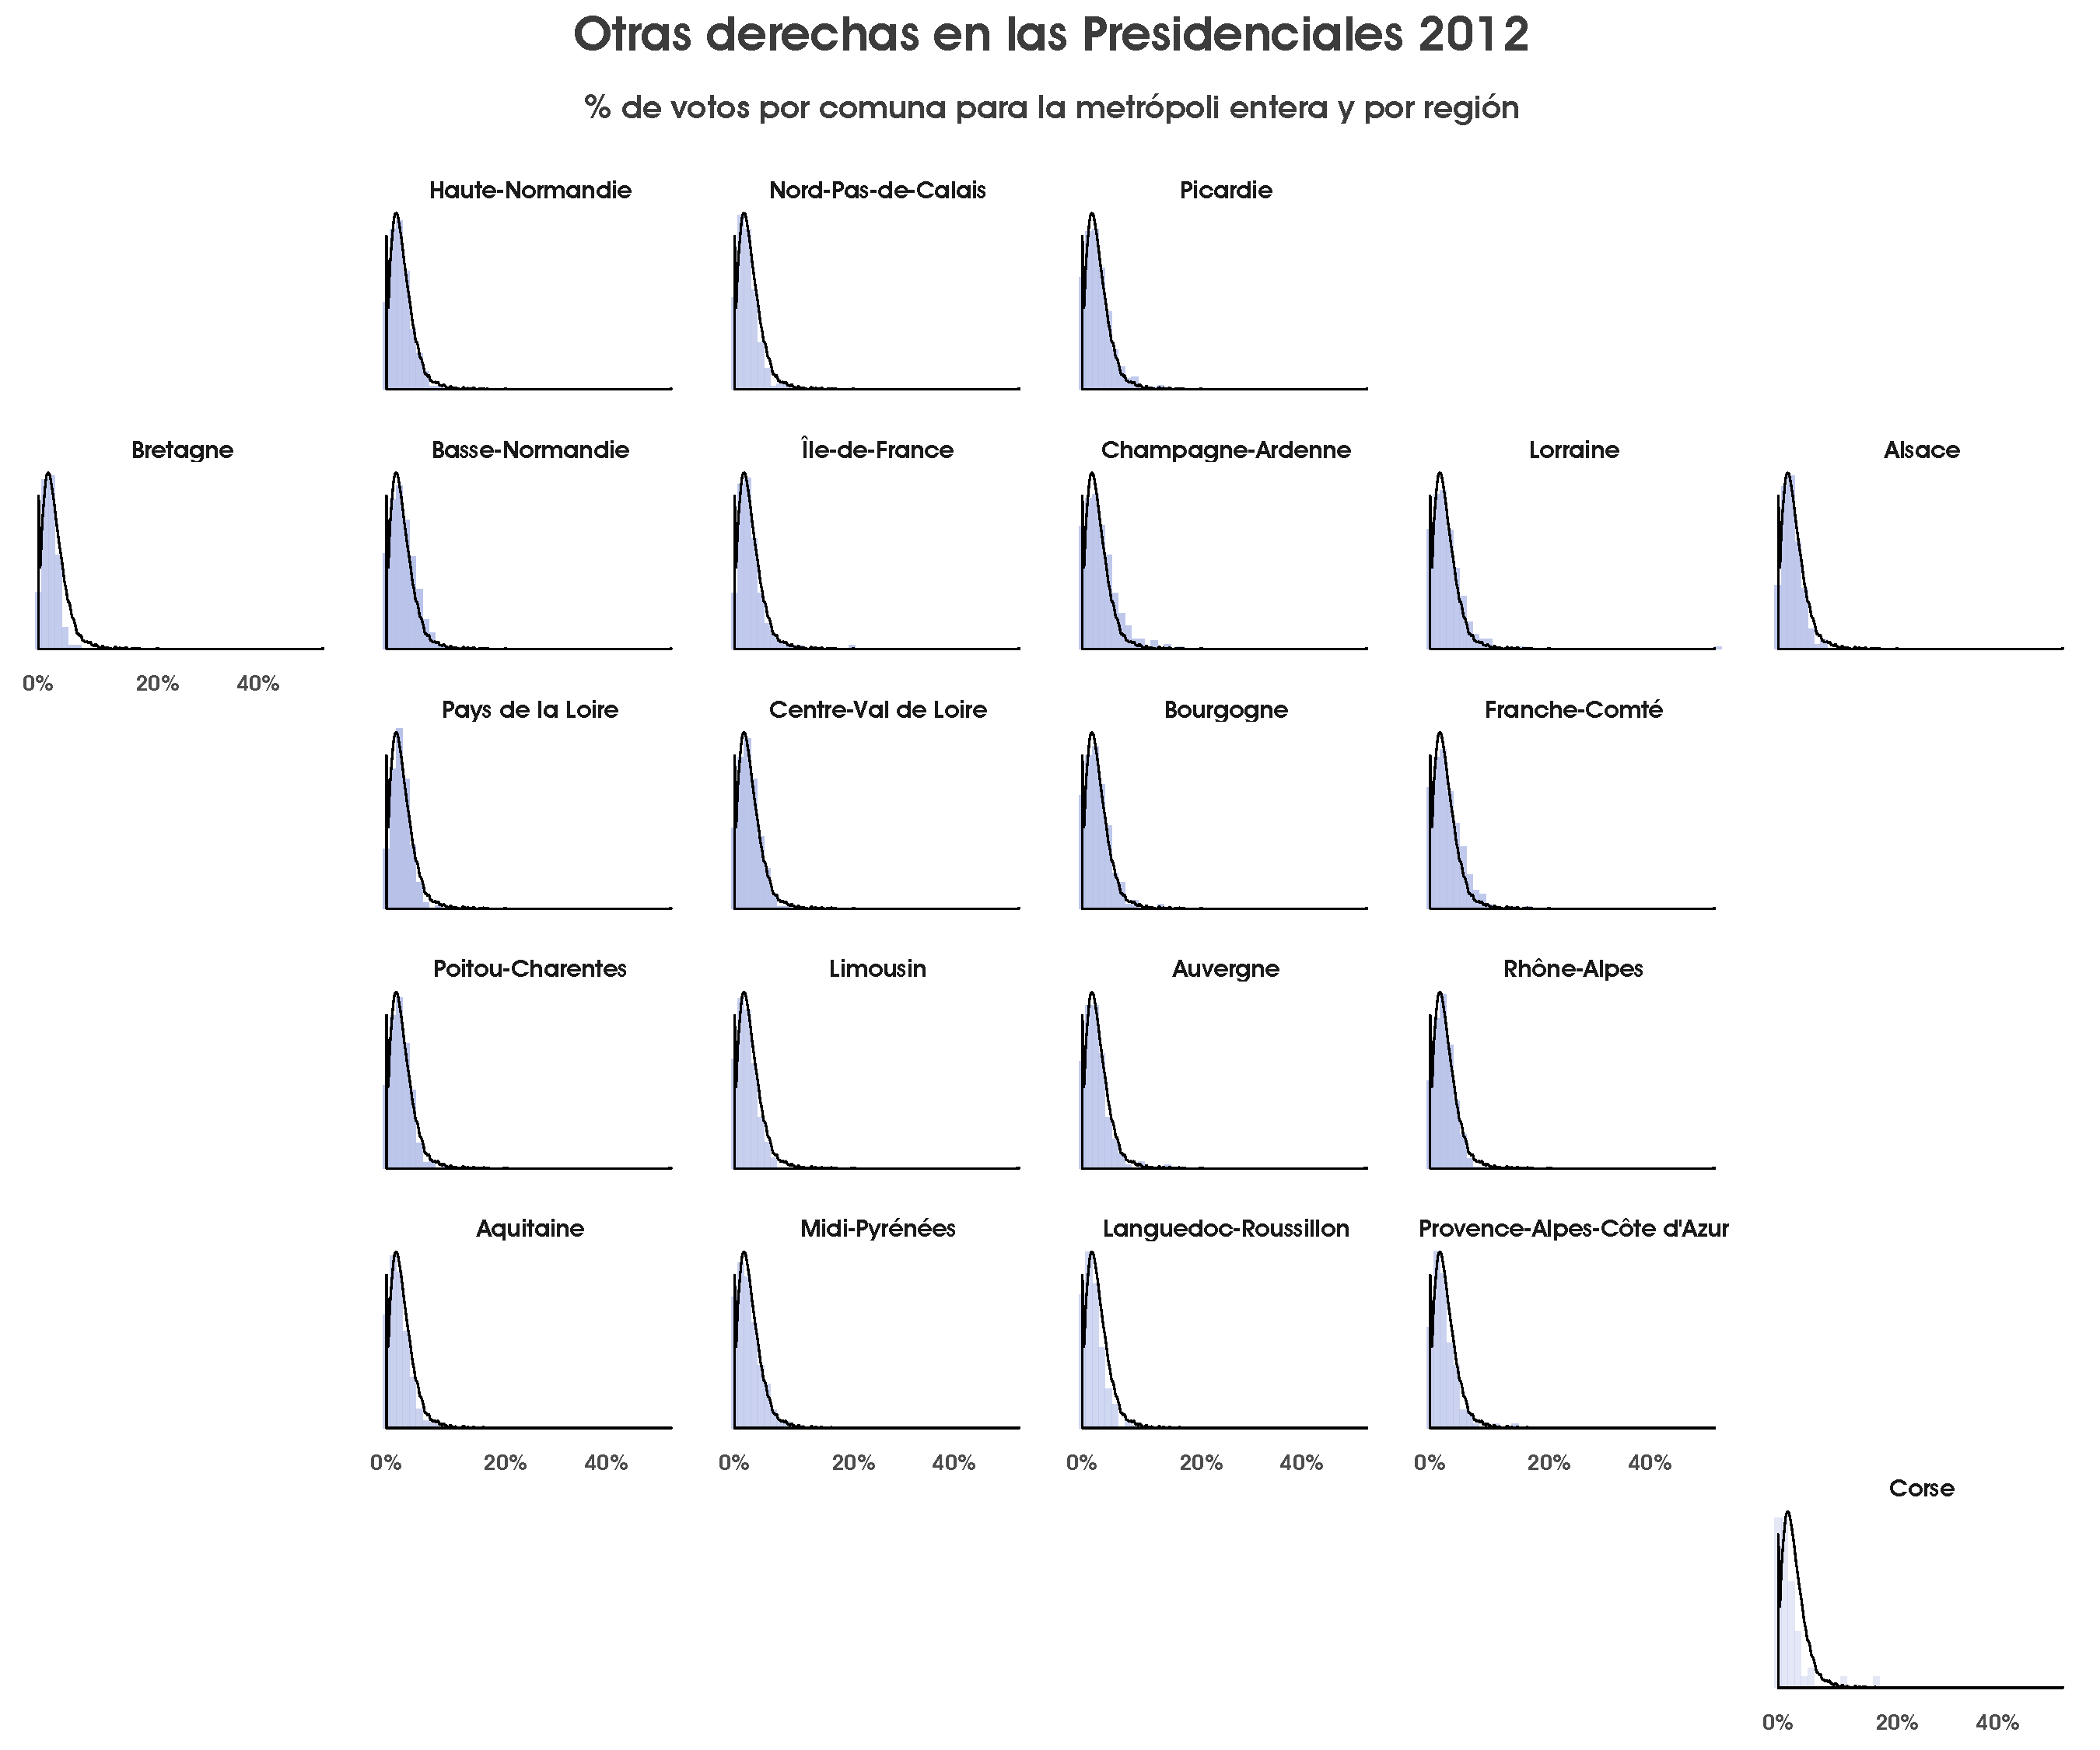
\includegraphics[width = \textwidth]{Figs/AED/Geofacet_Distr_por_Reg_P12_Otras_derechas}
	\end{subfigure}
	~
	\begin{subfigure}{0.3\textwidth}
	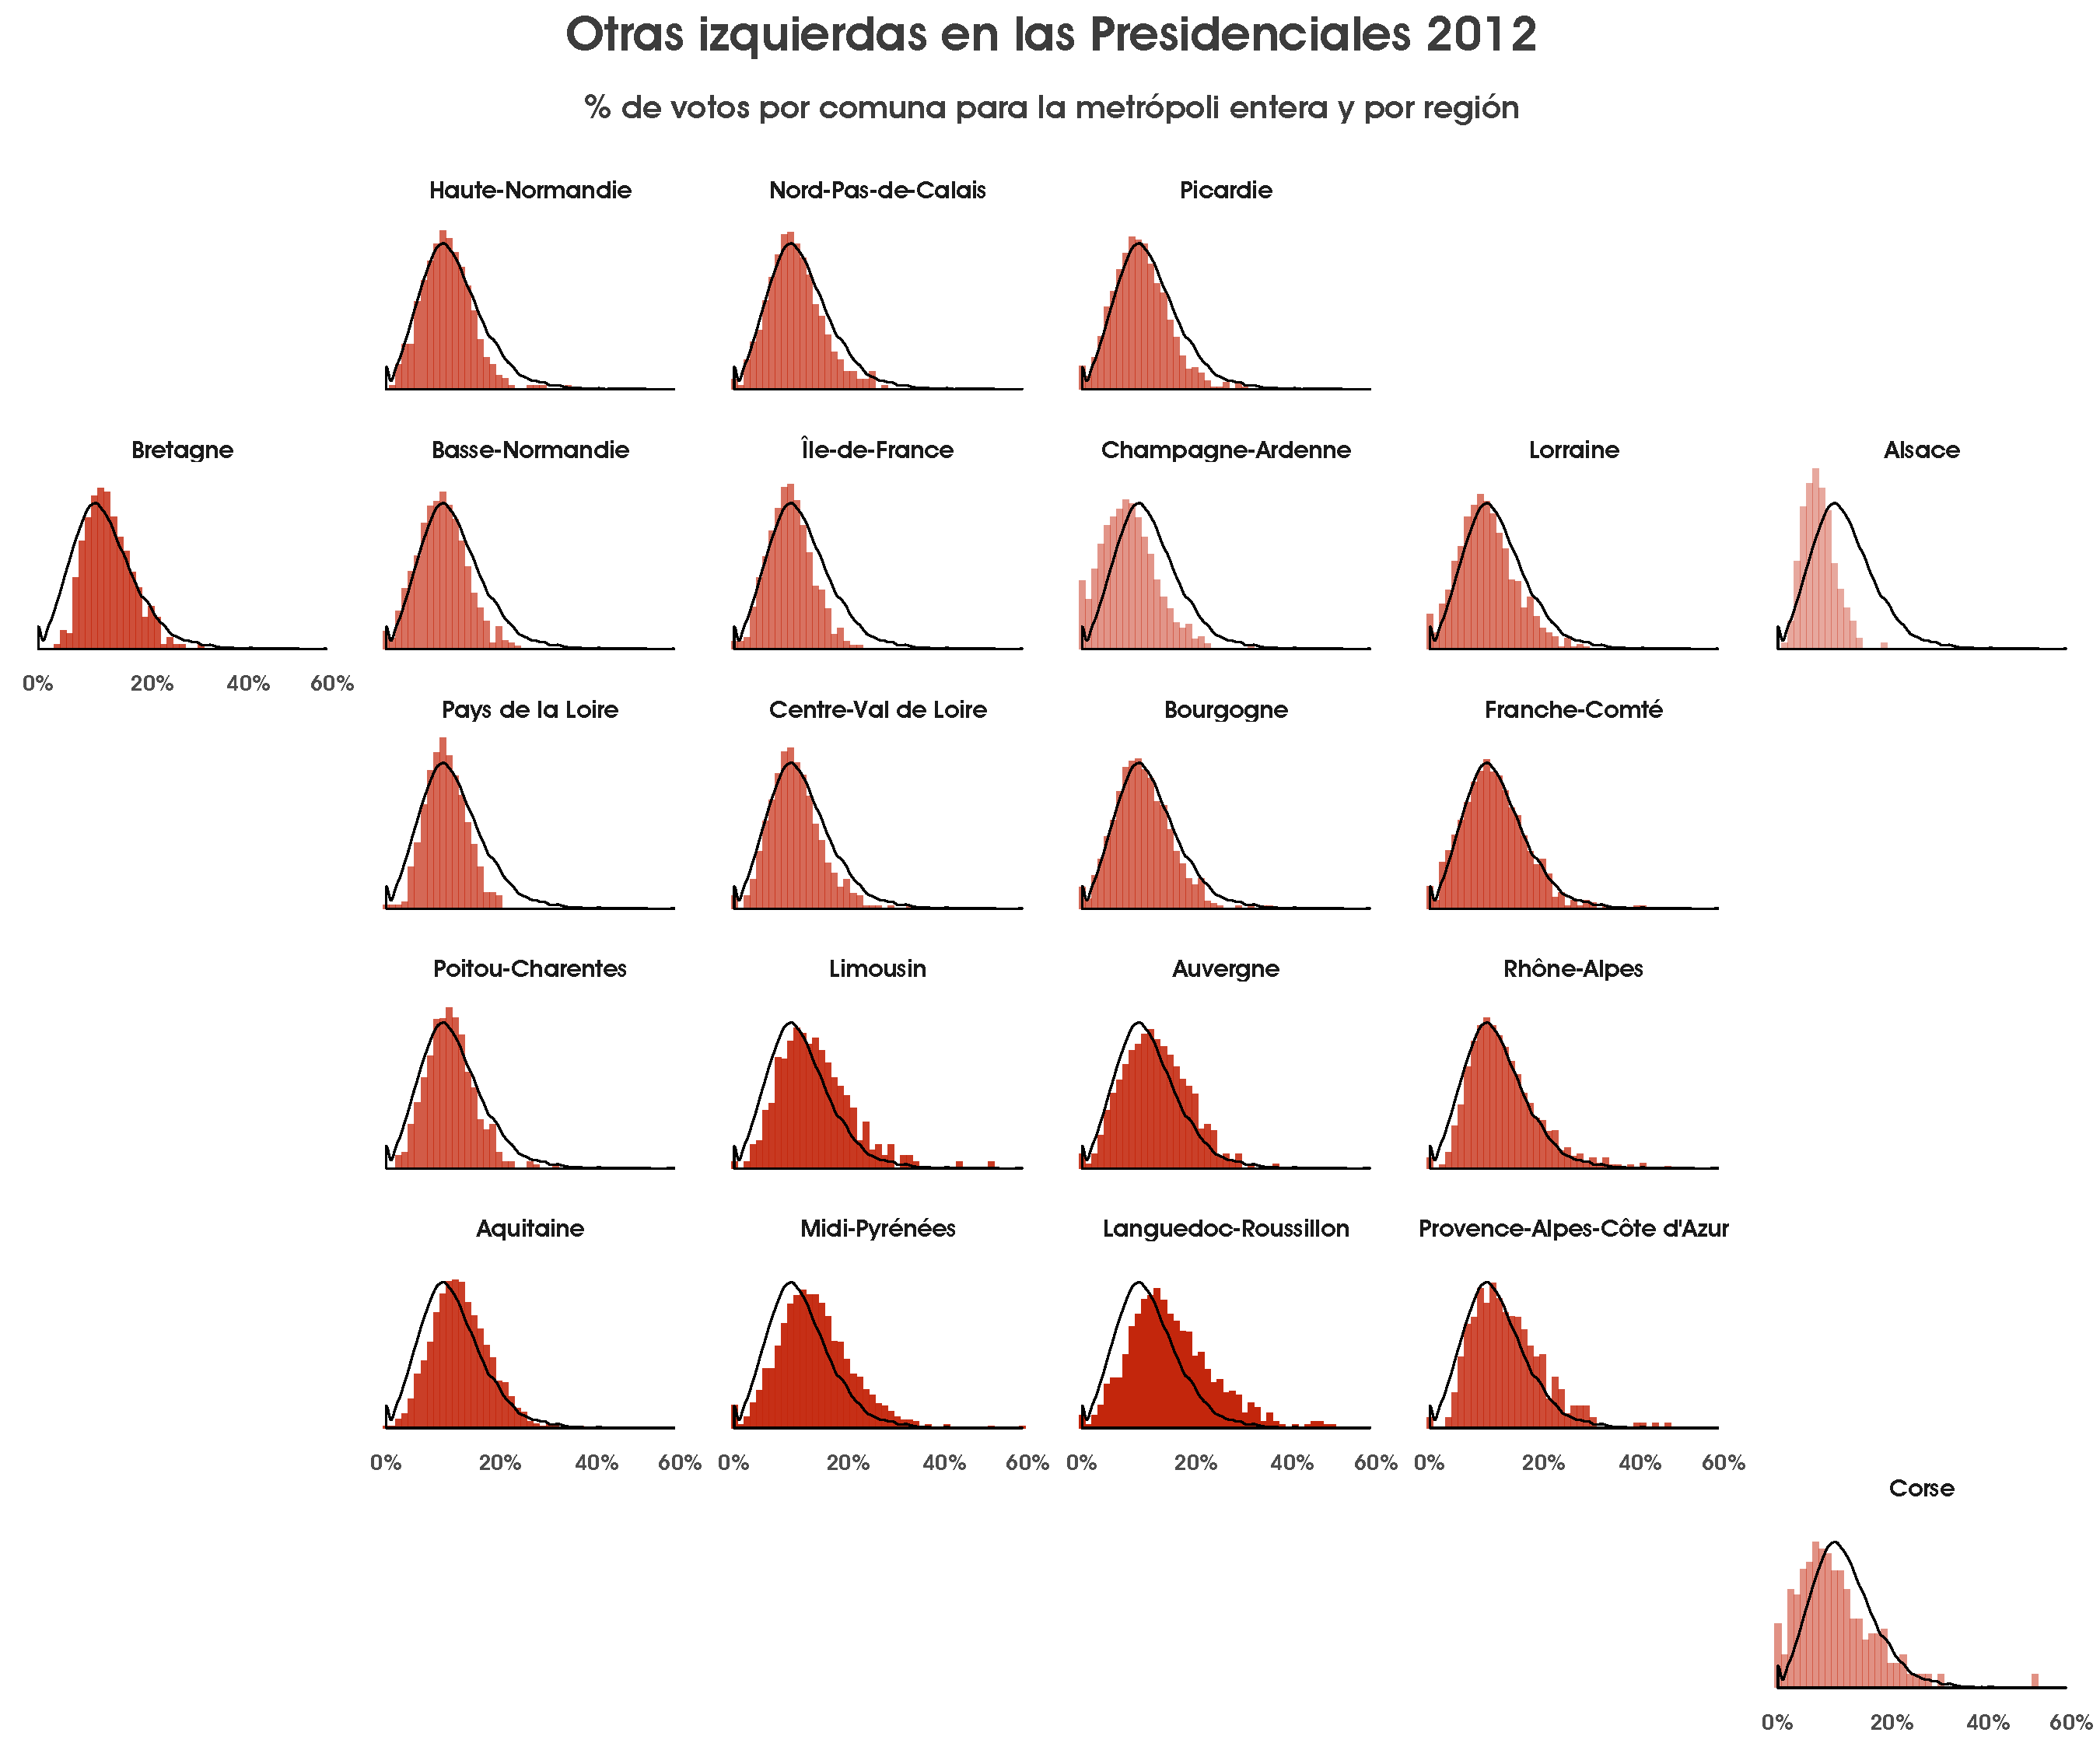
\includegraphics[width = \textwidth]{Figs/AED/Geofacet_Distr_por_Reg_P12_Otras_izquierdas}
	\end{subfigure}
	~
	\begin{subfigure}{0.3\textwidth}
	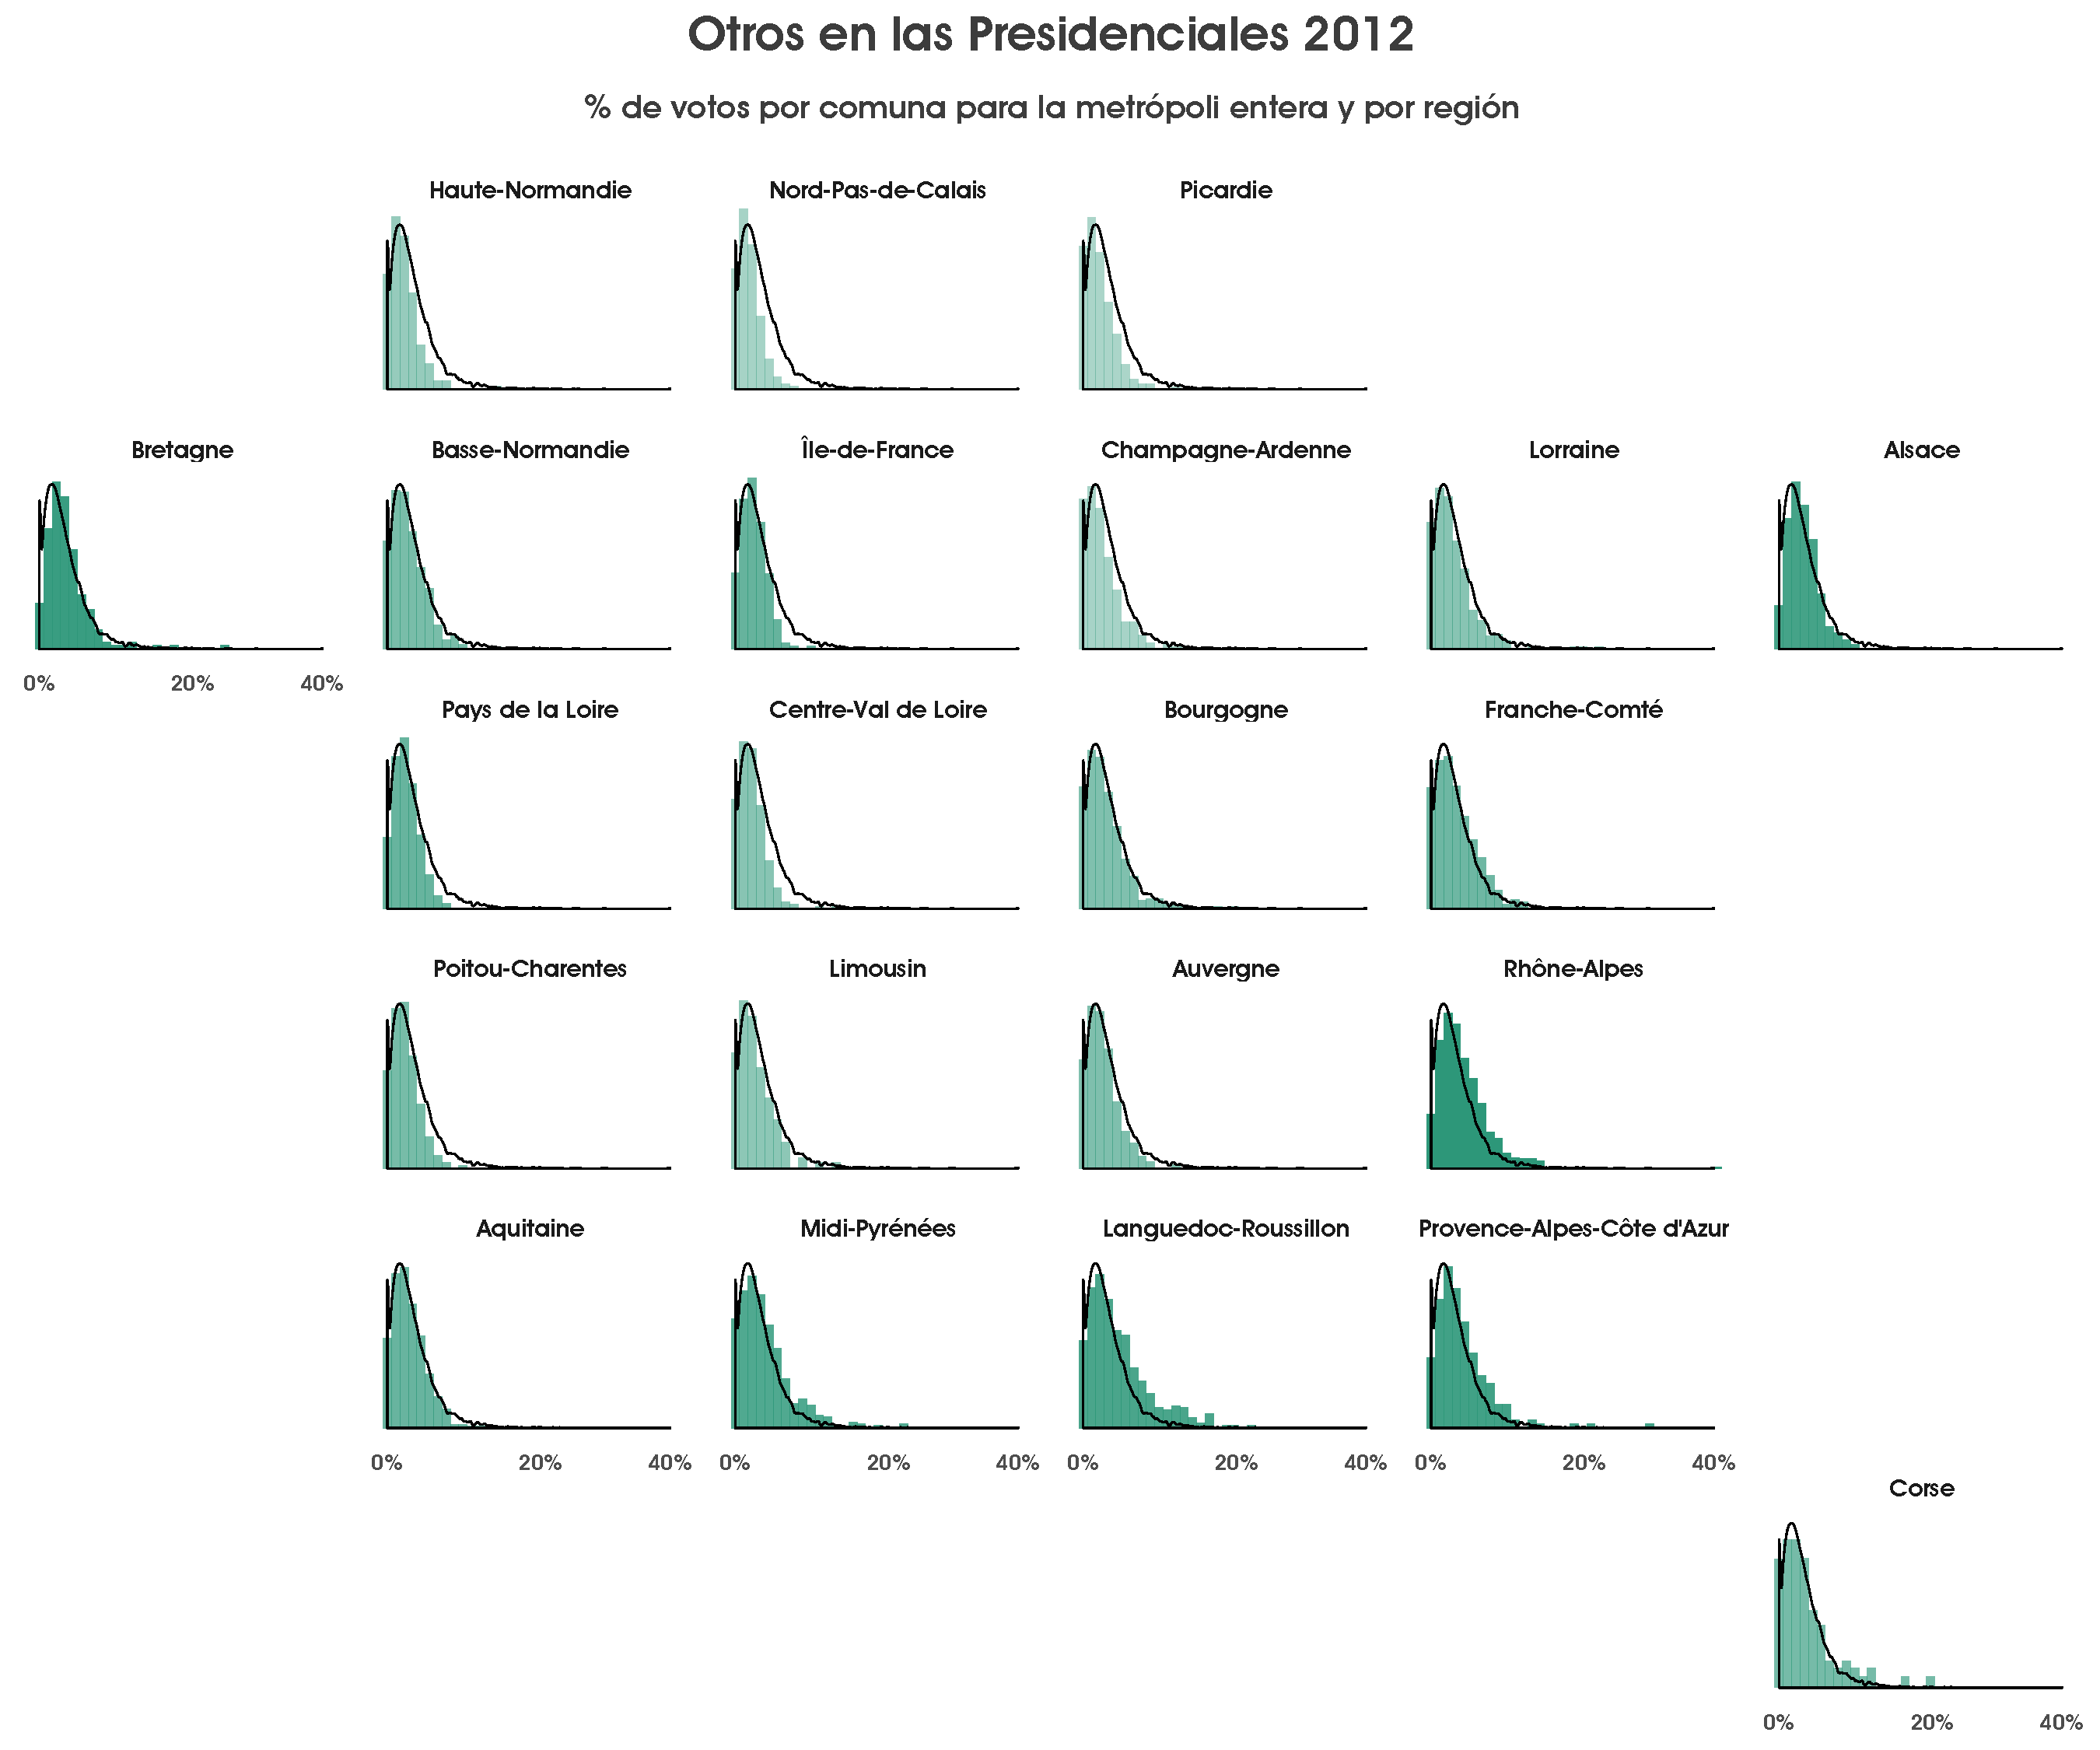
\includegraphics[width = \textwidth]{Figs/AED/Geofacet_Distr_por_Reg_P12_Otros}
	\end{subfigure}
	\caption{\textit{Geofacets} de la distribución del \% de votos obtenido por las 7 distintas etiquetas políticas en las elecciones presidenciales del 2012. Los histogramas representan la distribución de los porcentajes por comuna para cada una de las regiones. Las densidades transparentes representan la distribución de referencia considerando todas las comunas de la metrópoli francesa. La intensidad del color de los histogramas refleja la fuerza relativa de cada etiqueta en la región. Fuente: elaboración propia con base en los datos electorales oficiales del Ministerio del Interior francés.}
	\label{fig:Geofacet_Distr_Reg_P12}	
\end{figure}

Vemos que, en las regiones del noreste francés como Picardie o Alsace, los histogramas del FN están desplazados a la derecha de la distribución de referencia y, por tanto, están coloreados con mayor intensidad. Por el contrario, en regiones occidentales como Bretagne, Limousin o Aquitaine, los histogramas reflejan menores porcentajes de votos para el FN y, por ejemplo, mayores votos a la izquierda. Así pues, podemos empezar a conjeturar que una clave geográfica para el voto frontista es la diagonal que va de Normandía--- Haute y Basse Normandie--- hacia PACA\footnote{Provence-Alpes-Côtes d'Azur.}: si la comuna se encuentra al noreste de la diagonal, tendería a manifestar mayor apoyo al Front National que si se encuentra al sudoeste de la misma.\\ 

Podemos desagregar las distribuciones un nivel más y observarlas mediante diagramas de violines por departamento. Los \textit{geofacets} respectivos para el FN en las cuatro elecciones se observan en la \textbf{Figura \ref{fig:Geofacet_Distr_Dptos_FN}}. En cada región se muestran 3 líneas como referencia del rango intercuartílico y la mediana considerando las comunas de toda la metrópoli. El diagrama de violín sin relleno muestra dicha distribución agrupada para toda la metrópoli. Los diagramas de violín con relleno representan, pues, las distribuciones del porcentaje de votos obtenido en cada comuna del departamento correspondiente, identificado mediante su código oficial geográfico. Dentro de cada región los departamentos están ordenados de menor a mayor apoyo al FN con base en las medianas. Al igual que en los histogramas a nivel región, la intensidad del relleno es el cociente de la mediana departamental respecto a la mediana global.\\ 

\begin{figure}[h]
	\centering
	\begin{subfigure}{0.4\textwidth}
	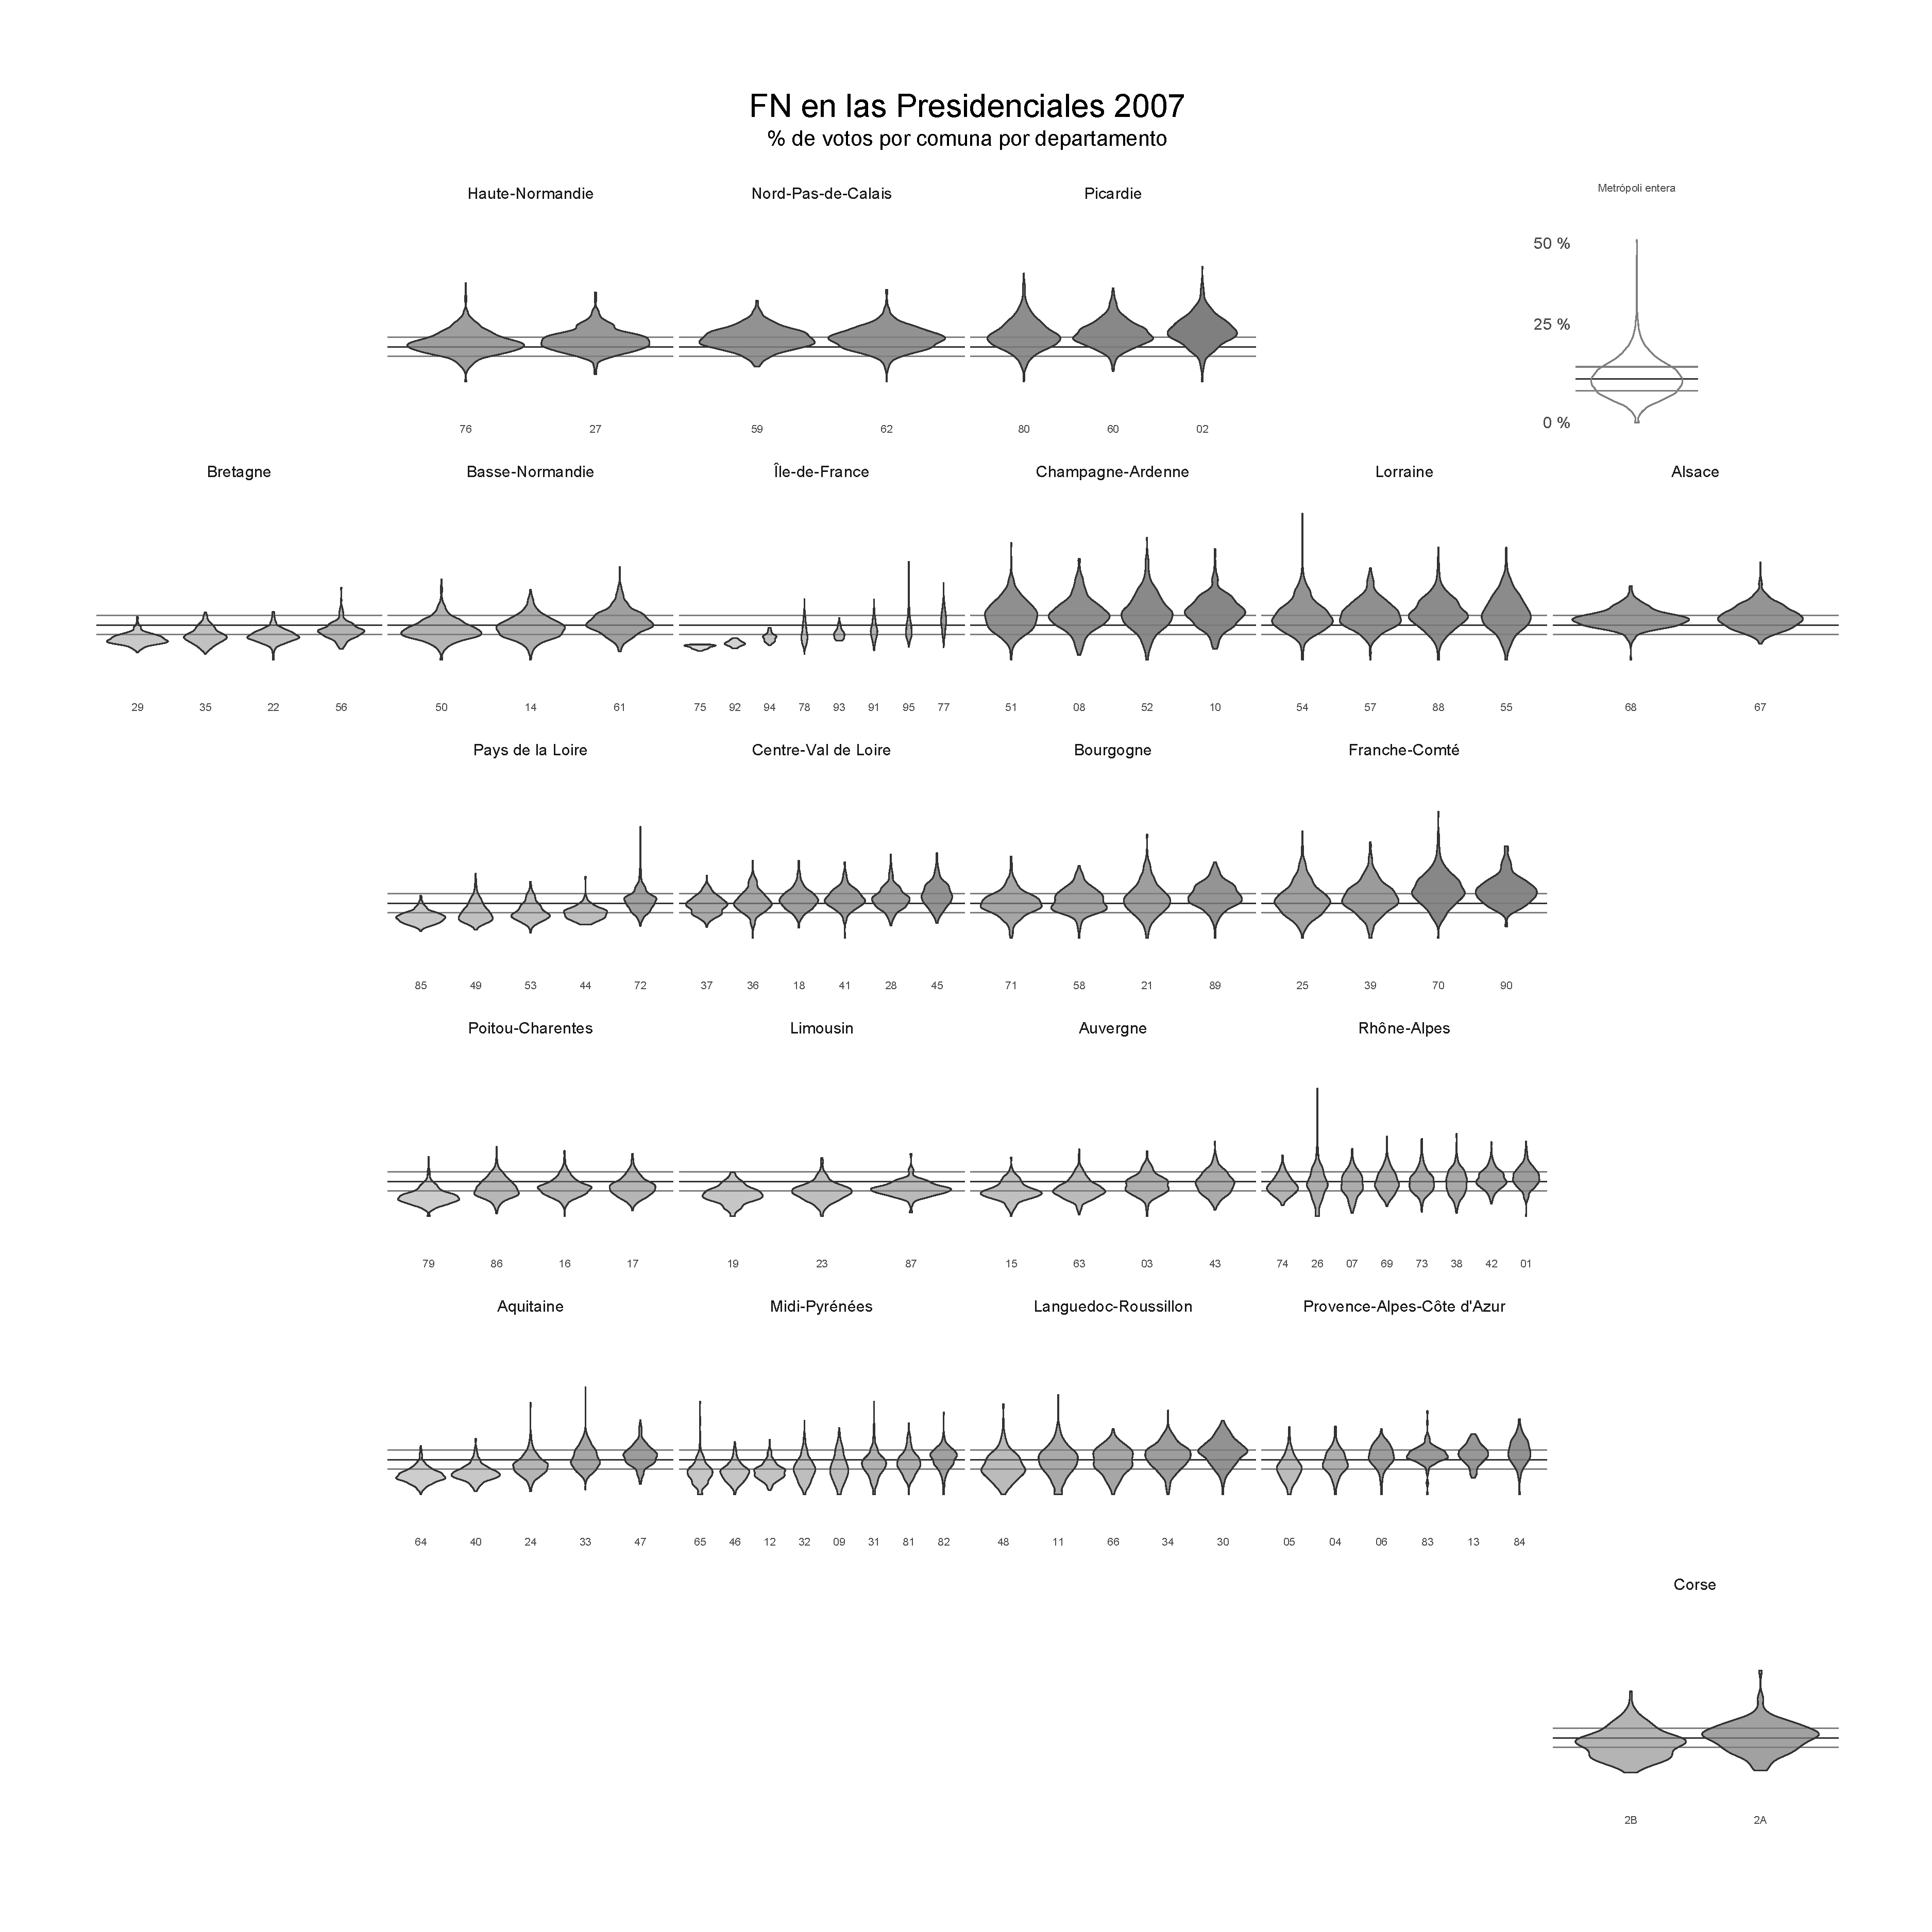
\includegraphics[width = \textwidth]{Figs/AED/Geofacet_Distr_por_Dpto_P07_FN}
	\end{subfigure}
	~
	\begin{subfigure}{0.4\textwidth}
	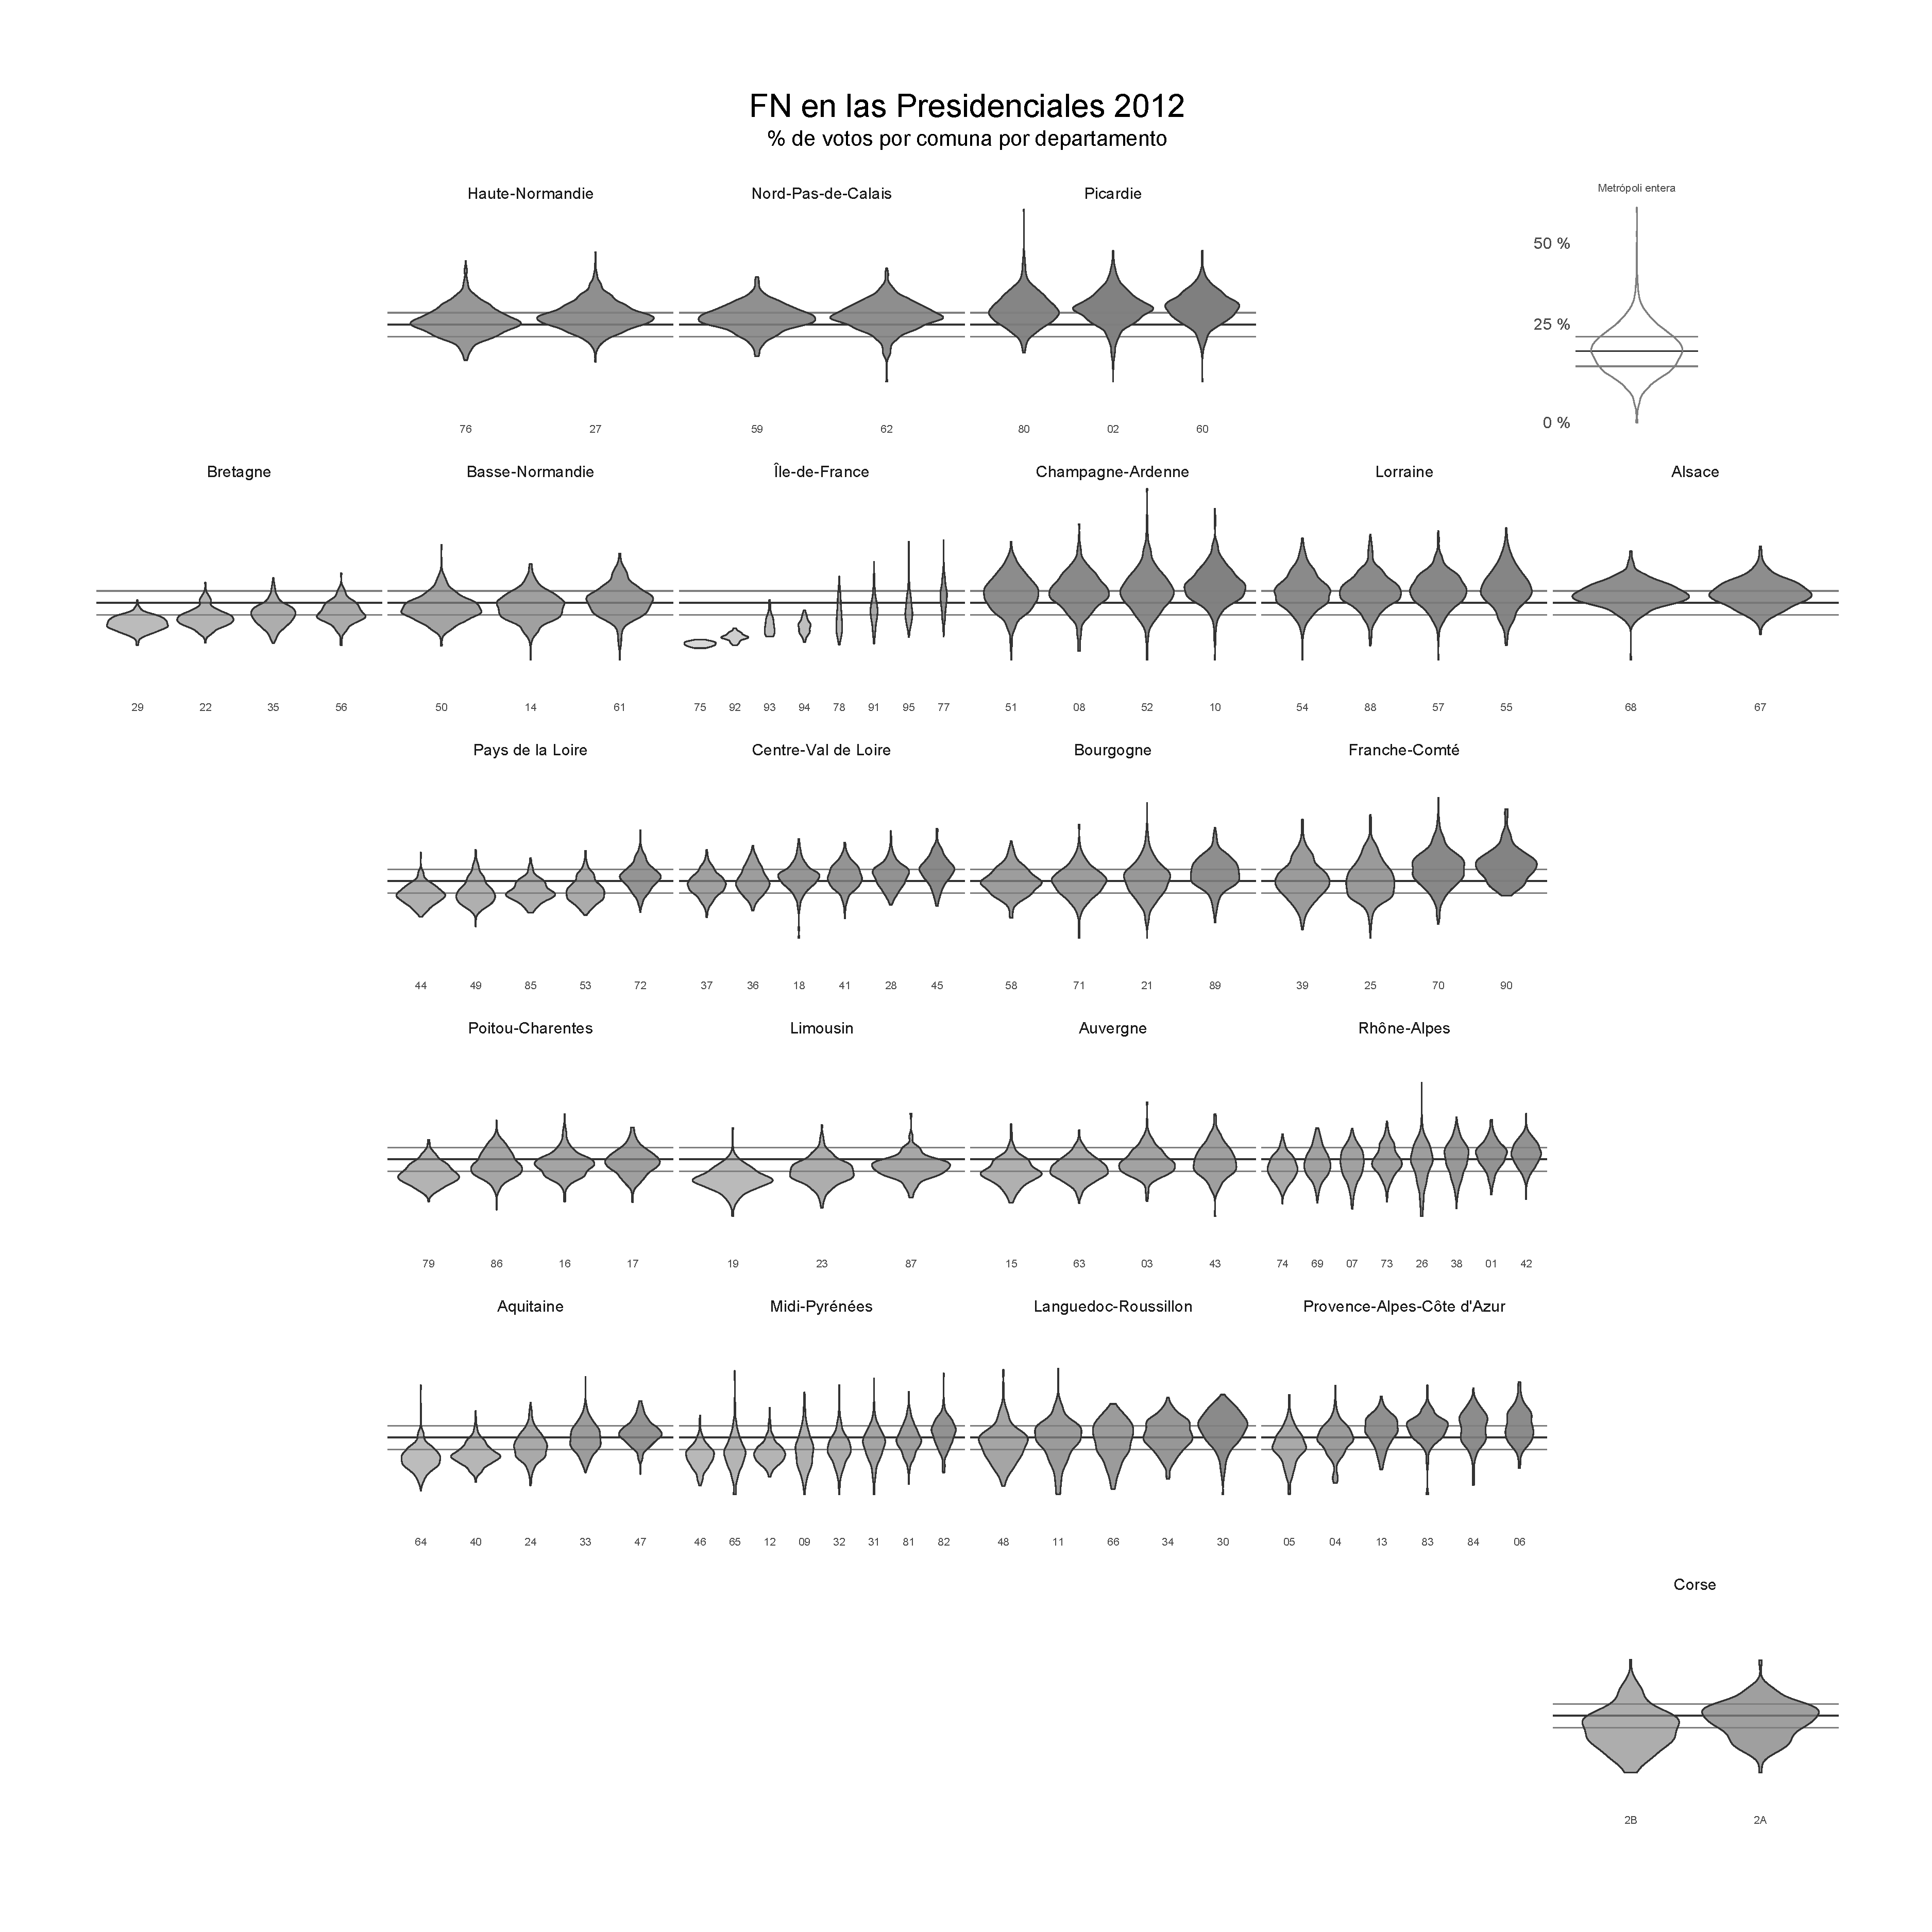
\includegraphics[width = \textwidth]{Figs/AED/Geofacet_Distr_por_Dpto_P12_FN}
	\end{subfigure}
	~
	\begin{subfigure}{0.4\textwidth}
	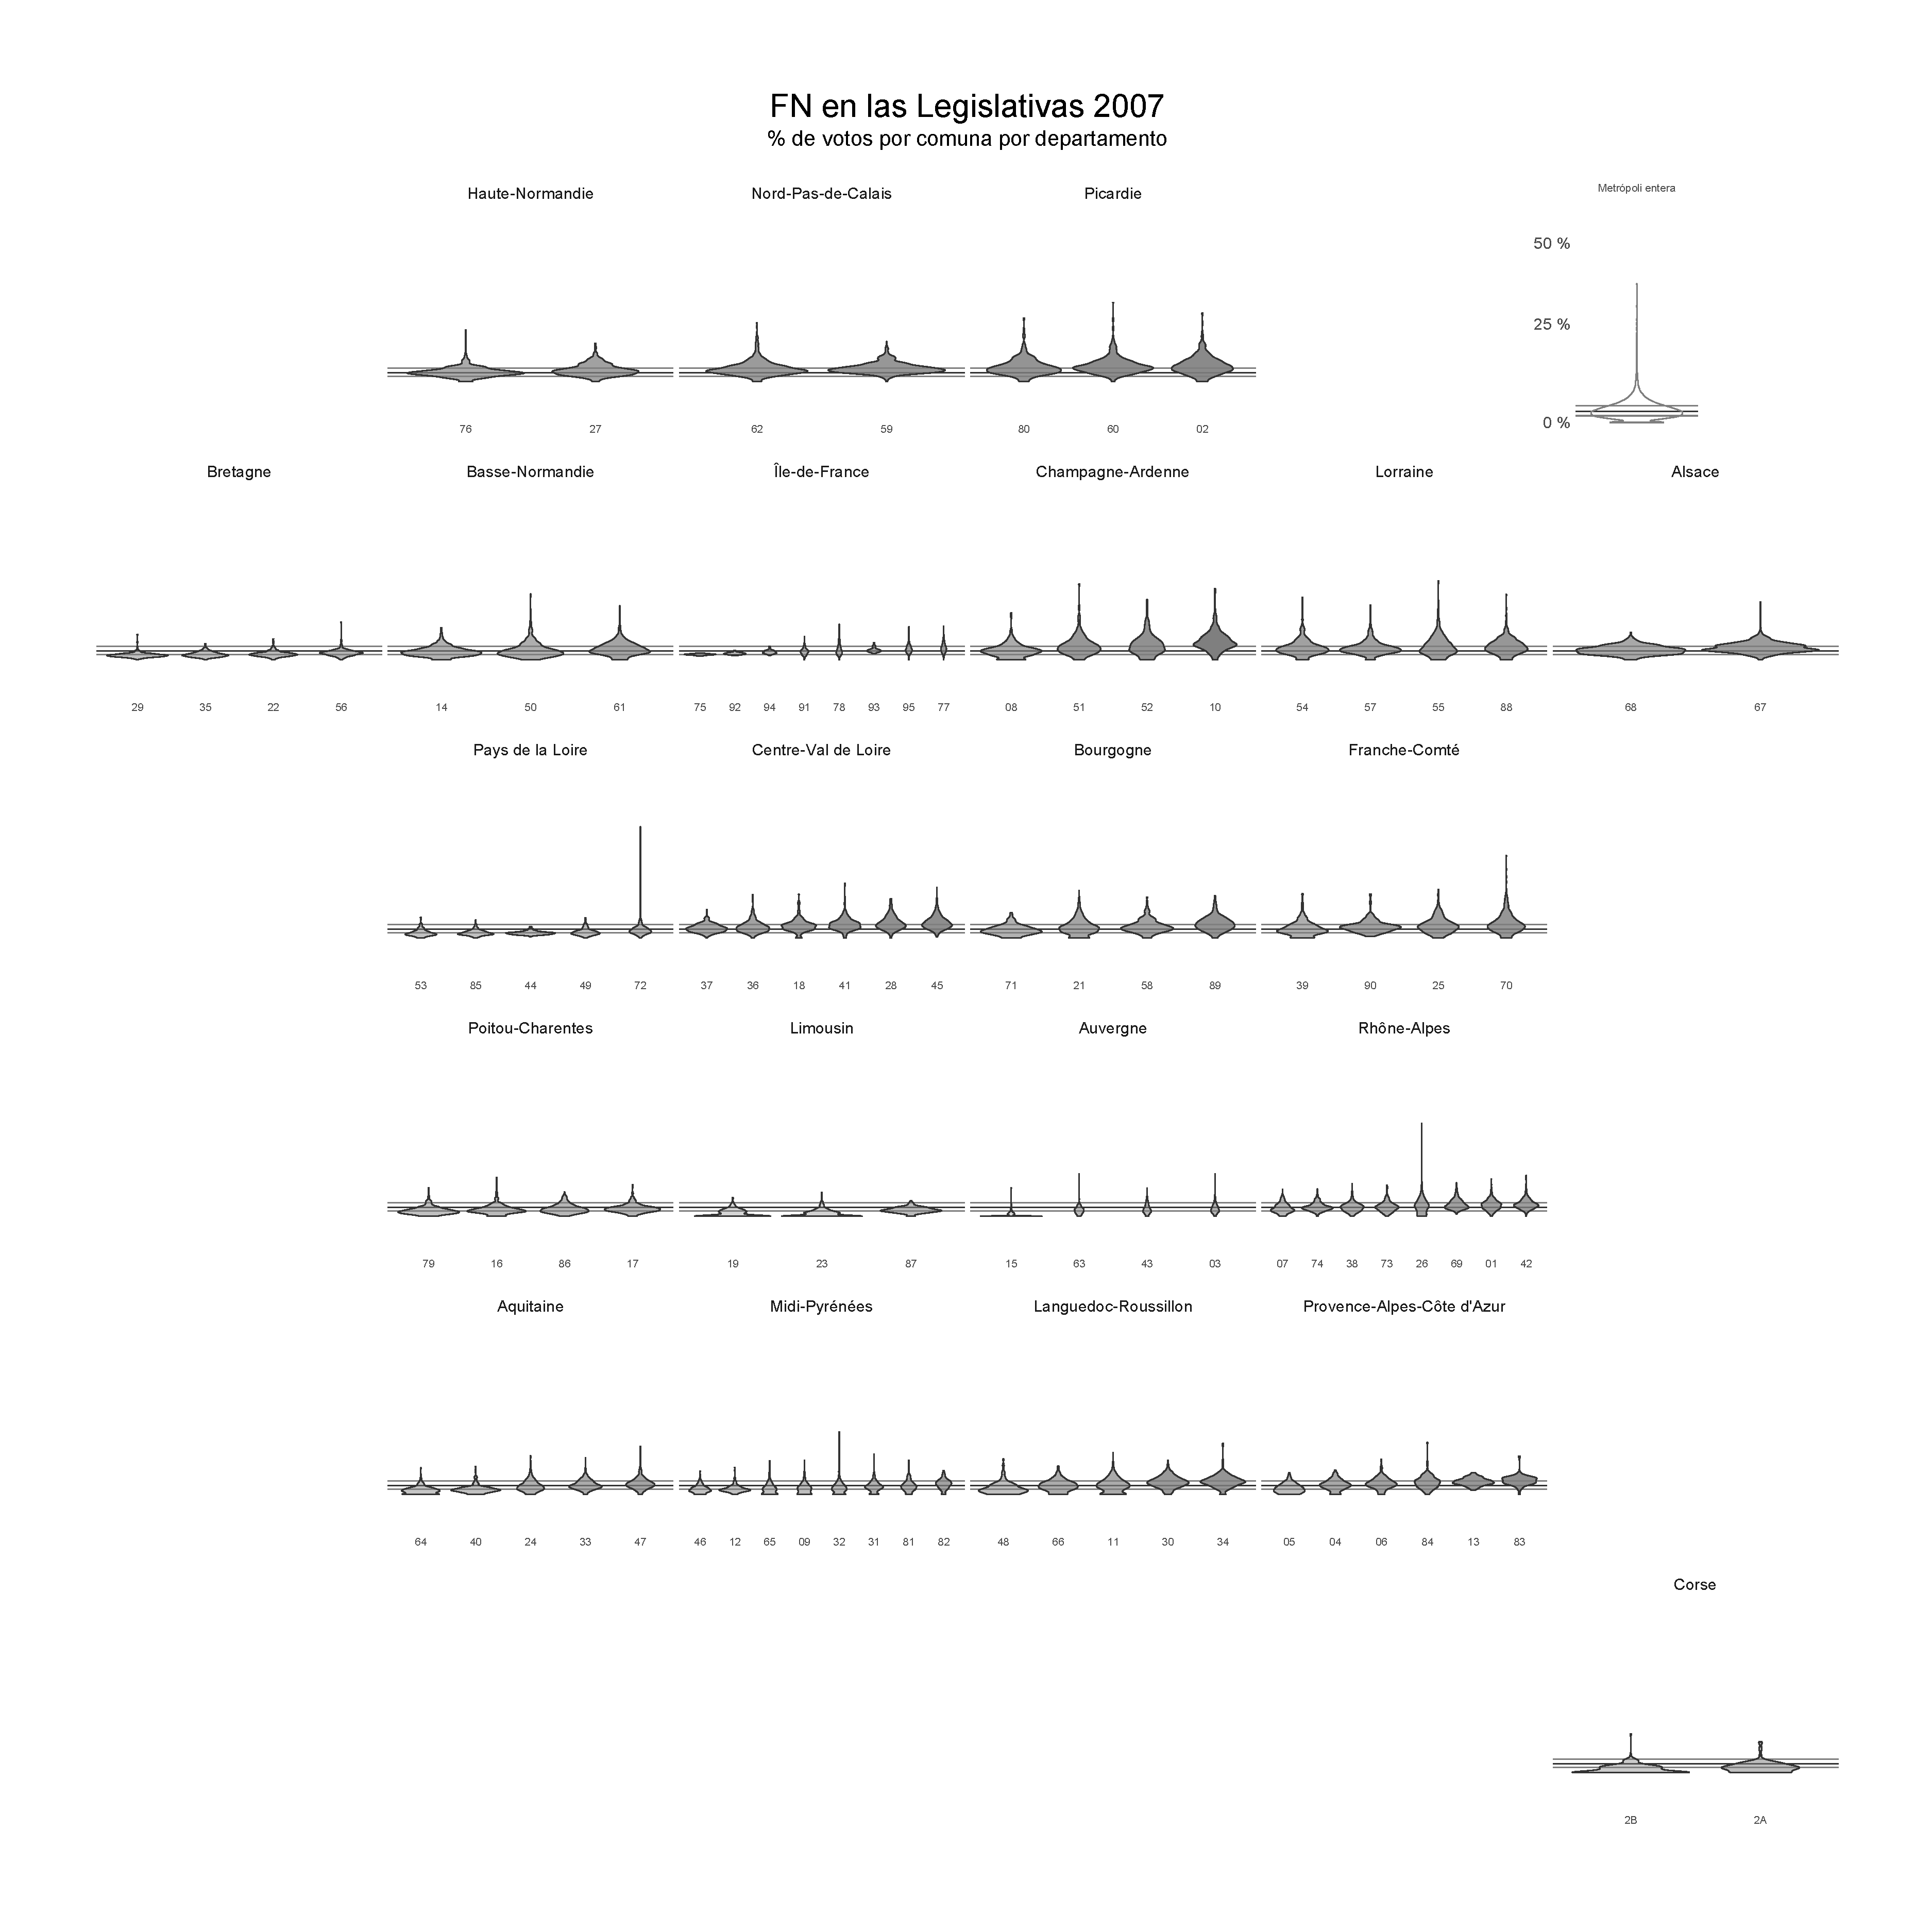
\includegraphics[width = \textwidth]{Figs/AED/Geofacet_Distr_por_Dpto_L07_FN}
	\end{subfigure}
	~
	\begin{subfigure}{0.4\textwidth}
	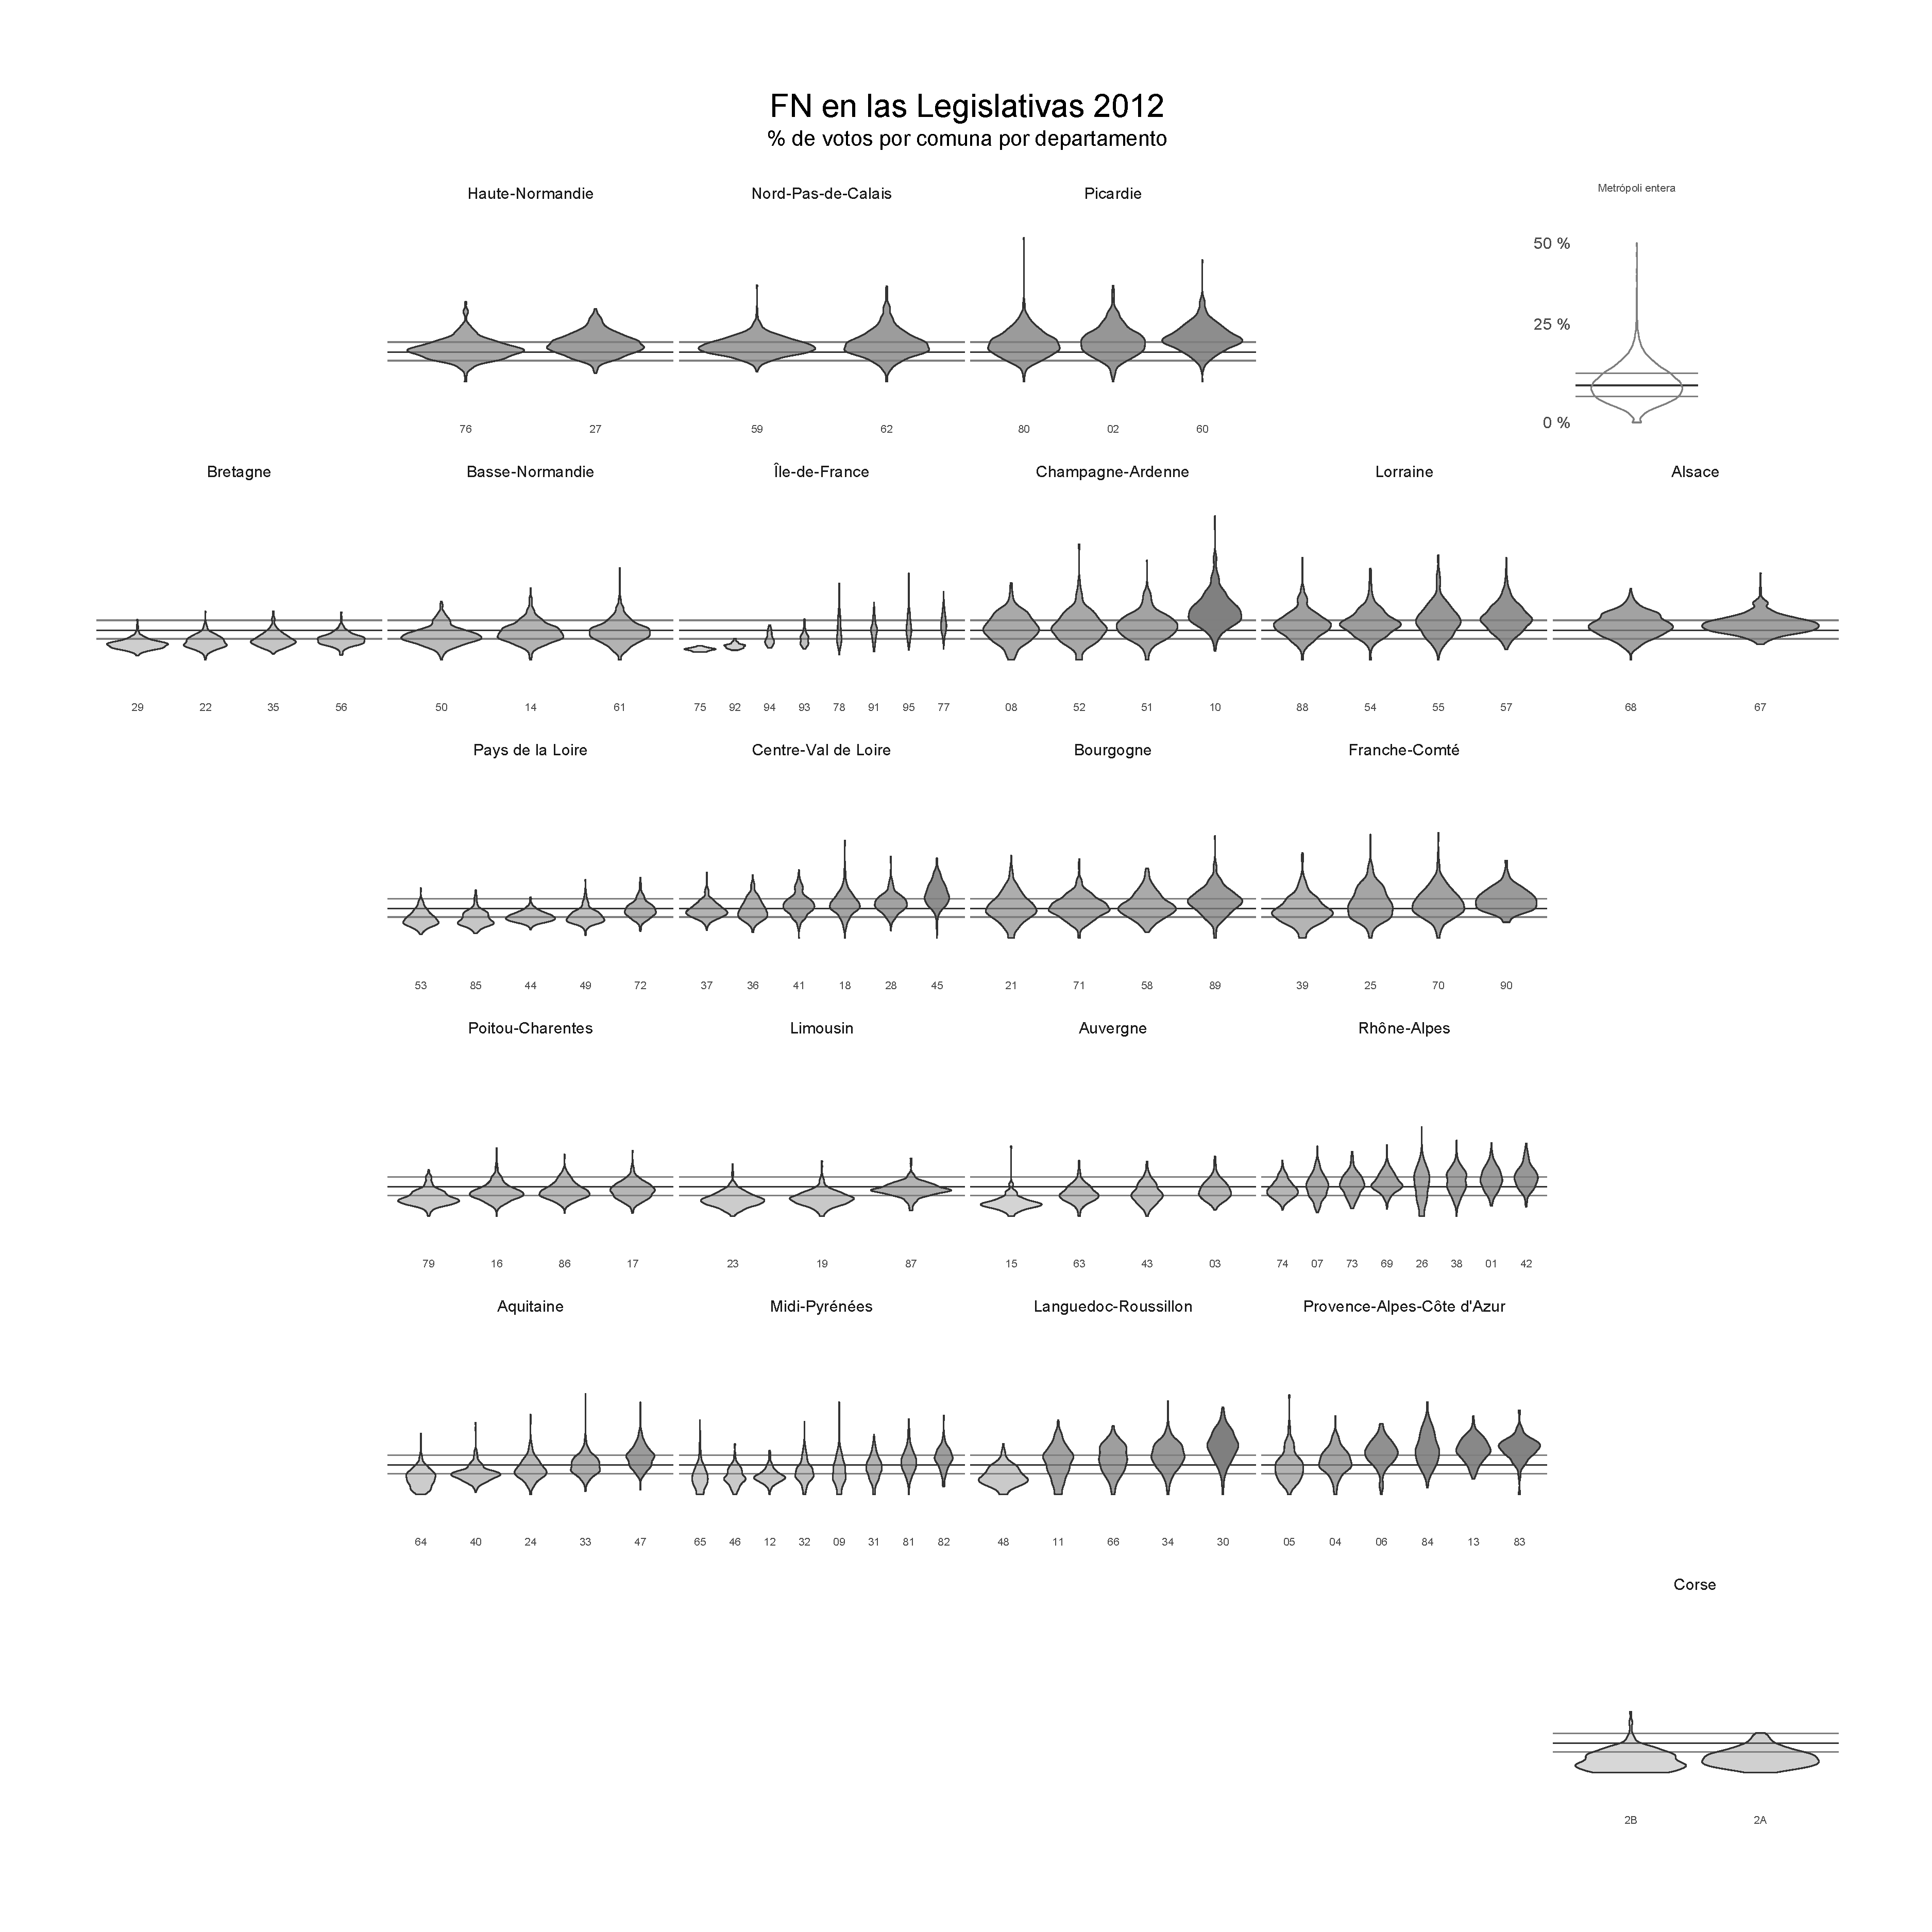
\includegraphics[width = \textwidth]{Figs/AED/Geofacet_Distr_por_Dpto_L12_FN}
	\end{subfigure}
	\caption{\textit{Geofacets} de la distribución del \% de votos obtenido por el FN en las 4 elecciones; presidenciales arriba, legislativas abajo. los violines rellenos de color son las distribuciones considerando solo las comunas del departamento correspondiente mientras que las 3 líneas horizontales representan una referencia al rango intercuartílico y la mediana de la distribución considerando todas las comunas de la metrópoli, misma que puede verse en el panel superior derecho. Fuente: elaboración propia con base en los datos electorales oficiales del Ministerio del Interior francés.}
	\label{fig:Geofacet_Distr_Dptos_FN}	
\end{figure}

Podemos notar algunas cosas. En primer lugar, es evidente que el FN sufre un efecto arrastre en las elecciones legislativas. Al ganar la presidencia un candidato de otro partido, dicha plataforma se ve beneficiada en las legislativas; por ello, el voto por las demás opciones disminuye, como es el caso del FN. Por otro lado, vemos que dentro de las regiones con mayor apoyo en general, este es relativamente homogéneo a través de los departamentos. En efecto, las distribuciones reflejadas en diagramas de violines para los departamentos dentro de Lorraine, Champagne-Ardenne o Picardie aparentan ser similares, salvo casos especiales como el departamento 10-Aube en las legislativas de 2012. No obstante, existen regiones--- como Île de France o Aquitaine--- cuyos departamentos presentan distribuciones más diferentes. Este es un elemento que podría empezar a sugerir un modelado jerárquico de los datos.